
% citep
% \section{TODO}
% %De ce que je comprends , les gens font surtout des variational auto encoder, ou du masking
% %Mentionner que la méthode proposé peut être utilisé avec des réseaux
% %\sam{Approche NTK, fédéré personalisation, projet avec Axel, Lien entre continuous normalizing flow}
% Plan intro: 
% \begin{itemize}
%     \item Representation of patterns in time series has several applications in biology, but halso for classification, deep learning finds features automaticly.
%      Taking or not taking into account time can be done with DTW. However, either the representation is the result of a black box and need post analysis to be understand,
%       which is difficult to apply statiscal tools on it, or the representation is desgned by hand to select relevant features, but the capacity of analysis is limited by the knowledge of the designer.
%      \item In shape analysis, representation of shapes for statistical analysis in a long time issue, which has been solved mainly by the LDDMM framework. Representing shapes as diffeomorpshims of a common shape. 
%      \item However, this tool has not been yet applied on time series, even if there is already some tools developped for oriented curves. 
%      \item In this work, we propose to apply LDDMM to time series and to show its interest to derive an interpretable and unsupervised representation of patterns in time series.
%      We proposed some tools developped in the shape analysis community to the researcher interested in machine learning and time series ones.
%      \item First, we introduce our assumptions regarding the dataset and the main problem of diffeomorpshim learning. Then, we show how to solve it with LDDMM .
%       We expose how to apply it to time series by selecting wisely a RKHS kernel, motivating it with a representation theorem.
%       experiments on synthetic data are presented to show that the parameter of representation are identifiable when the time seriess are not too sharp and the kernels parameter well tuned. 
%       Then, we sh-ow how to apply the method on an unsupervised case of moouse respeitaory dataset and a supervised one on ... .

% \end{itemize}

% One option to tackle this issue is to derive ...
% feature representation of time series which depends on the problem at hand.
% which is parti... -> which is of prime interest in ...
\vspace{-1ex}
\section{Introduction}
\vspace{-1ex}
%https://arxiv.org/abs/1811.00075
%Appliqué sur les "UWaveGestureLibrary","ArticularyWordRecognition","Cricket" pour l'archive UEA
%"ArrowHead", "BME", "ECG200","FacesUCR","GunPoint" dans le cas univarié

%Idée de parler d'inter individualité, spécialiser davantage
%k shape, shapelets , ye2009time


Our goal is to analyze the inter-individual variability within a time series dataset, an approach of significant interest in physiological contexts \cite{guscelli2019importance, wang2016research, bar2012studying, germain2023unsupervised}.
 Specifically, we aim to develop an unsupervised feature representation method that encodes the specificities of individual time series in comparison to a reference time series.
In physiology, examining the various "shapes" in a time series related to biological phenomena and their variations due to individual differences or pathological conditions is common.
 However, the term "shape" lacks a precise definition and is more intuitively understood as the silhouette of a pattern in a time series. In this paper, we refer to the shape of a time series as the graph of this signal.

 Although community structures with representatives can be learned in an unsupervised manner \cite{trirat2024universal, meng2023unsupervised} using contrastive loss \cite{franceschi2019unsupervised, tonekaboni2021unsupervised, meng2023unsupervised} or similarity measures \cite{asgari2023clustering, germain2023unsupervised, paparrizos2015k, ye2009time},
  the study of inter-individual variability of shapes within a cluster \cite{niennattrakul2007inaccuracies, shirato2023identifying} remains an open problem in unsupervised representation learning (URL), particularly for \textit{irregularly sampled} time series with \textit{variable lengths}.
   
Our work explicitly focuses on learning shape-based representation of time series.
First, we propose to view the shape of a time series not merely as its curve $\{s_t:\eqsp t\in\msi\}$, but as its graph $\msg(s)=\{(t,s(t)):\eqsp t\in \msi\}$.
   Then, building on the shape analysis literature \cite{beg2005computing,vaillant2004statistics}, we adopt the Large Deformation Diffeomorphic Metric Mapping (LDDMM) framework \cite{beg2005computing,vaillant2004statistics} to analyze these graphs.
    The core idea is to represent each element $\msg(s^j)$ of a dataset $(s^j)_{j\in[N]}$ as the transformation of a reference graph $\msg(\mathbf{s}_0)$ by a diffeomorphism $\phi_j$, i.e. $\msg(s^j) \sim \phi_j . \msg(\mathbf{s}_0)$ .
    The diffeomorphism $\phi_j$ is learned by integrating an ordinary differential equation parameterized by a Reproducing Kernel Hilbert Space (RKHS).
     The parameters $(\alpha_j)_{j\in[N]}$ encoding the diffemorphisms $(\phi_j)_{j\in[N]}$ yield the representation features of the graphs $(\msg(s^j))_{j\in[N]}$.
     Finally, these shape-encoding features can be used as inputs to any statistical or machine-learning model.

However, a graph time series transformation by a general diffeomorphism is not always a graph time series, see e.g. \Cref{fig:diffeo}, thus a graph time series is more than a simple curve \cite{glaunes2008large}.
 Our contributions arise from this observation: we specify the class of diffeomorphisms to consider and show how to learn them.
  This change is fruitful in representing transformations of time series graphs as illustrated in \Cref{fig:transport}.
   %In this regard, this work is not an application of LDDMM to 1D curves \cite{glaunes2008large}.

     %In particular, the method can handle \textit{irregularly sampled} time series with \textit{variable sizes}.

    %  Our contributions can be summarized as follows:
    %  \begin{itemize}
    %    \item We propose an unsupervised method (TS-LDDMM) to analyze inter-individual variability of shapes in a time series dataset. In particular, the method can handle \textit{irregularly sampled} time series with \textit{variable sizes}.
    %    \item We motivate our extension of LDDMM to time series by introducing a theoretical framework with a representation theorem for time series graph (\Cref{theorem:representation}) and kernels related to their structure (\Cref{lemma:choice_of_kernel_V}).
    %    \item We demonstrate the identifiability of the model by estimating the true generating parameter of synthetic data, and we highlight the sensitivity of our method with respect to its hyperparameters, also providing guidelines for tuning.
    %    We highlight the \textit{interpretability} of TS-LDDMM for studying the inter-individual variability in a clinical dataset.
    %     We illustrate the quantitative interest of the representation on classification tasks on real shape-based datasets.
        
    %  \end{itemize}
    Our contributions can be summarized as follows:
    \begin{itemize}
       \item We propose an unsupervised method (TS-LDDMM) to analyze the inter-individual variability of shapes in a time series dataset (\Cref{section:methodology}). In particular, the method can handle multivariate time series \textit{irregularly sampled} and with \textit{variable sizes}.
       \item We motivate our extension of LDDMM to time series by introducing a theoretical framework with a representation theorem for time series graph (\Cref{theorem:representation}) and kernels related to their structure (\Cref{lemma:choice_of_kernel_V}).
       \item We demonstrate the identifiability of the model by estimating the true generating parameter of synthetic data, and we highlight the sensitivity of our method concerning its hyperparameters (\Cref{appendix: settings_identifiability}), also providing guidelines for tuning (\Cref{appendix:kernel_TS_LDDMM}).
       \item We highlight the \textit{interpretability} of TS-LDDMM for studying the inter-individual variability in a clinical dataset (\Cref{section:experiments}).
        \item We illustrate the quantitative interest of such representation on classification tasks on real shape-based datasets with regular and irregular sampling (\Cref{appendix: robustness}-\ref{appendix: settings_classification}).
 \end{itemize}

    %To the best of our knowledge, these theoretical and practical works have never been done before.
      % On synthetic data, we show the sensibility of the results according to the kernel parameters and give guidelines to tune it.
      % In an unsupervised framework, we vectorize respitory patterns of a mouse dataset and analyze the variations depending on the drug taken by the mouse.
      % Finally, we compare to the state-of-the-art methods in classification an ... classifier taking as inputs the representation given by LDDMM.
      
  %    \paragraph*{Related papers}
  %    %https://arxiv.org/pdf/2106.00750.pdf look to the related papers
  %  In the shape analysis community, a famous paper \cite{srivastava2010shape} addresses the problem of representation of curves $C:\msi \to \Rset^d$ by using the Square-Root Velocity (SRV) representation.
  %      This structure is particularly relevant to compute geodesics and distances between curves when the space is quotiented by time reparametrization.
  %       However, in our case the time axis deserves a particular attention, since the curves are derived from time-series. 
  %       %While \cite{srivastava2010shape} tackles the computations of geodesics and distances on quotient curves space, our aim is to get a vector representation of each pattern. 
  %       Very recently, in \cite{heo2024logistic}, this representation was used to compute PCA and to perform classification on quotient curves space, we follow the same ideas, but we focus on time series and we use LDDMM instead of SRV.
 % optimization framework with a well chosen neural architecture in order to learn automatically the features, which has been very 
% To understand these complex data, we are looking to simpler representations toperform classical statiscal analysis or to perform efficient downstream tasks of machine learning, the time series representation res time series to a real valued vector representation. in order to apply classical statiscal or machine learning tools depending on the needs such as Principal Component Analysis (PCA), logistic regression or deep learning methods for classification or anomaly detection.

% \thi{
%   Our goal is to analyze the inter-individual variability within a time series dataset, an approach of prime interest in physiological contexts \cite{guscelli2019importance,wang2016research,bar2012studying,germain2023unsupervised}. More specifically, we aim to find an unsupervised features representation method that encodes individual time series specificities compared to a reference one.
% }

% \thi{
%   Studying shape differences between time series related to biological mechanisms is a common practice in physiology to characterize healthy and pathological functioning CITE. For instance, the shapes of heartbeats in electrocardiograms are discriminant for some cardiovascular pathologies CITE. Several approaches have been proposed for such comparison. Some employ shape-based similarity measures between time series \cite{asgari2023clustering,germain2023unsupervised,paparrizos2015k,ye2009time},  others embed time series as vectors of predefined features CITE, and, with the rise of deep neural networks, unsupervised learning representation of time series~\cite{trirat2024universal,meng2023unsupervised} has shown to be a valuable approach CITE notably with contrastive learning~\cite{franceschi2019unsupervised,tonekaboni2021unsupervised,meng2023unsupervised}. However, shape-based representation of time series within cohorts~\cite{niennattrakul2007inaccuracies,shirato2023identifying} remains an open problem in URL.
% }

% \thi{
%   Our work focuses explicitly on learning shape-based representation of time series. First, we propose not to see the shape of a time series through its curve $\{s_t:\eqsp t\in\msi\}$, but rather through its graph $\msg(s)=\{(t,s(t)):\eqsp t\in \msi\}$.
%    Then, building on the shape analysis literature \cite{beg2005computing,vaillant2004statistics}, we follow the Large Deformation Diffeomorphic Metric Mapping (LDDMM) framework \cite{beg2005computing,vaillant2004statistics} to analyze these graphs. The idea is to represent each element $\msg(s^j)$ of a dataset $(s^j)_{j\in[N]}$ as the transformation of a reference graph $\msg(\mathbf{s}_0)$ by a diffeomorphism $\phi_j$ (ie $\msg(s^j) \sim \phi_j . \msg(\mathbf{s}_0)$ ).
%     The diffeomorphism $\phi_j$ is learned by integrating an ordinary differential equation parameterized by a Reproducing Kernel Hilbert Space (RKHS).
%      The parameters $(\alpha_j)_{j\in[N]}$ encoding the diffemorphisms $(\phi_j)_{j\in[N]}$ yield the representation features of the graphs $(\msg(s^j))_{j\in[N]}$. Finally, these shape-encoding features can feed any statistical or machine-learning model.
%   }

% \thi{
%   However, a graph time series transformation by a general diffeomorphism is not always a graph time series, see e.g. \Cref{fig:diffeo}, thus a graph time series is more than a simple curve \cite{glaunes2008large}. Our contributions arise from this observation: we specify the class of diffeomorphisms to consider and show how to learn them. This change is fruitful in representing transformations of time series graphs as illustrated in \Cref{fig:transport}.
% }

% \thi{
%   Our contributions can be summarized as follows:
%     \begin{itemize}
%        \item We propose an unsupervised method (TS-LDDMM) to analyze the inter-individual variability of shapes in a time series dataset. In particular, the method can handle multivariate time series \textit{irregularly sampled} and with \textit{variable sizes}.
%        \item We motivate our extension of LDDMM to time series by introducing a theoretical framework with a representation theorem for time series graph (\Cref{theorem:representation}) and kernels related to their structure (\Cref{lemma:choice_of_kernel_V}).
%        \item We demonstrate the identifiability of the model by estimating the true generating parameter of synthetic data, and we highlight the sensitivity of our method concerning its hyperparameters, also providing guidelines for tuning.
%        \item We highlight the \textit{interpretability} of TS-LDDMM for studying the inter-individual variability in a clinical dataset.
%         \item We illustrate the quantitative interest of such representation on classification tasks on real shape-based datasets.
%  \end{itemize}
% }

\begin{figure}[t]
  \centering
  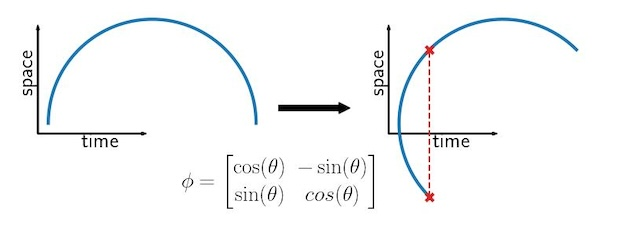
\includegraphics[width=0.7\linewidth]{"./pictures/diffeo.jpeg"}
  
  \caption{A time series' graph $\msg=\{(t,s(t)): \eqsp t\in\msi\} $ can lose its structure after applying a general diffeomorphism $\phi.\msg$: a time value can be related to two values on the space axis.}
  \label{fig:diffeo}
  
\end{figure}

\begin{figure*}[t]
  \centering
  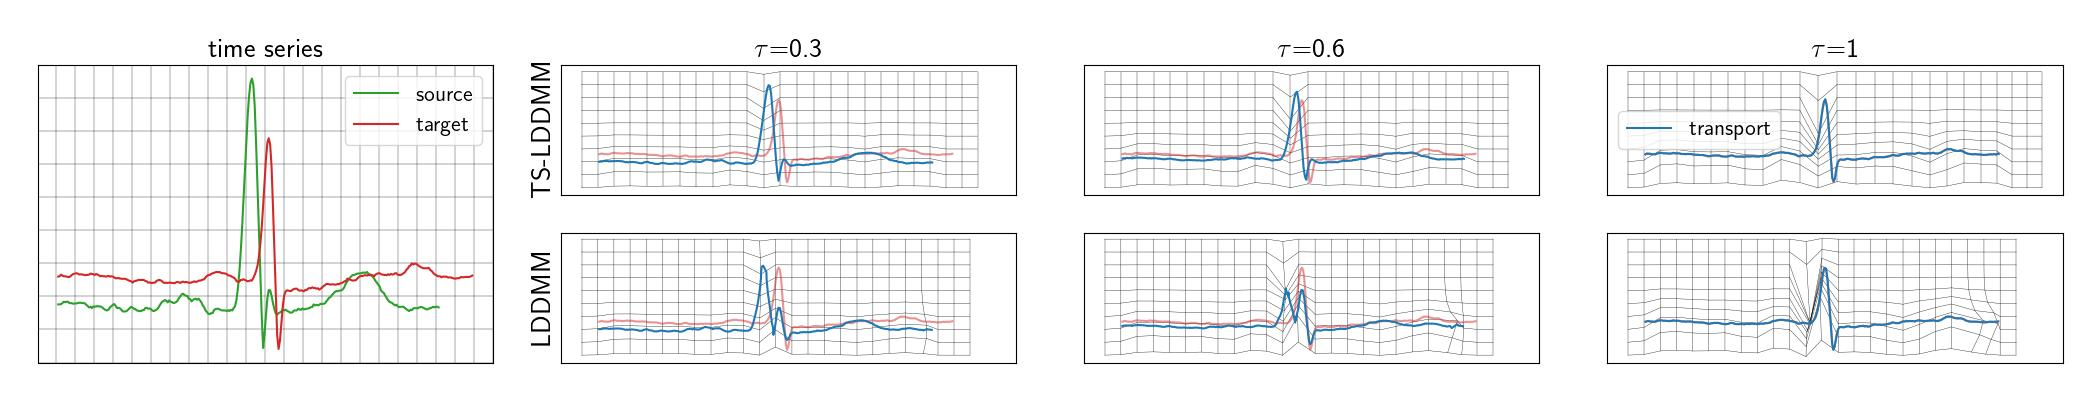
\includegraphics[width=\linewidth]{"./pictures/transport.jpeg"}
  
  \caption{LDDMM and TS-LDDMM are applied to ECG data.
  We observe that LDDMM, using a general Gaussian kernel, does not learn the time translation of the first spike but changes the space values, i.e., one spike disappears before emerging at a translated position. At the same time, TS-LDDMM handles the time change in the shape.
  This difference of \textit{deformations} implies differences in features \textit{representations}.   }
  \label{fig:transport}
  
\end{figure*}

  \vspace{-1ex}
\section{Notations}
We denote by integer ranges by $[k:l]=\{k,\ldots,l\}\subset \mathcal{P}(\Zset)$ and $ [l]=[1:l]$ with $k,l\in \Nset$,
by $\rmC^m(\msi,\mse)$ the set of $m$-times continously differentiable function defined on an open set $\msu$ to a normed vector space $\mse$,
 by $||u||_\infty=\inf_{x\in \msu} |u(x)| $ for any bounded function $u:\msu \to \mse$,
and by $\Nset_{>0}$ is the set of positive integers. 
%We are in a sub class of curve quotiented by temporal reparametrisation since a time series' graph can be understood as the equivalent class of t ->(t,s(t))

%Reproducing Kernel Hilbert Space (RKHS)
\vspace{-1ex}
\section{Background on LDDMM}
\vspace{-1ex}
\label{section:LDDMM}

In this part, we expose how to
 learn the diffeomorphisms $(\phi_j)_{j\in[N]}$ using LDDMM, initially introduced in \cite{beg2005computing}.
 In a nutshell, for any $j\in [N]$, $\phi_j$ corresponds to a differential flow related to a learnable velocity field belonging to a well-chosen Reproducing Kernel Hilbert Space (RKHS).

 In the next section, time series are going to be represented by diffeomorphism parameters $(\alpha_j)_{j\in[N]}$.
 That is why LDDMM is chosen since it offers a parametrization for diffeomorphisms that is sparse and interpretable, two features particularly relevant in the biomedical context.
 

The basic problem that we consider in this section is the following. Given a set of targets $\mathbf{y}=(y_i)_{i\in[T_2]}$ in $\Rset^{d'}$\footnote{Note that we denote by $d'\in\nset$ the ambient space}, a set of starting points $\mathbf{x}=(x_{i})_{i\in[T_1]}$ in $\Rset^{d'}$, we aim to find a diffeomorphism $\phi$ such that the finite set of points $\mathbf{y}$ is similar in a certain sense to the set of finite sets of transformed points $\phi \cdot \mathbf{x} =(\phi(x_i))_{i\in[T_1]} $.
 The function $\phi$ is occasionally referred to as a \textit{deformation}. In general, these sets $\mathbf{x},\mathbf{y}$ are meshes of continuous objects, e.g., surfaces, curves, images, and so on.

 \vspace{-1ex}
% LDDMM is designed to analyzed an existing dataset, while NF and CNF are made to generalize a dataset for data augmentation.
\paragraph{Representing diffeomorpshims as deformations.}
Such \textit{deformations} $\phi$ are constructed via differential flow equations, for any $x_0\in \Rset^{d'} $ and $\tau\in[0,1]$:
\begin{equation}
  \label{eq:LDDMM_dynamic}
    \frac{\dd X(\tau)}{\dd \tau}= v_\tau(X(\tau)), \quad X(0)=x_0\eqsp ,
    \phi^v_\tau(x_0)=X(\tau), \quad \phi^v=\phi^v_1  \eqsp ,
\end{equation}
where the velocity field is $v:\tau\in [0,1]\mapsto v_\tau\in \msv $
and $\msv$ is a Hilbert space of continuously differentiable function
on $\Rset^{d'}$.  If
$||\dd u ||_{\infty}+|| u ||_{\infty}\leq ||u ||_\msv $ for any
$u\in \msv$ and
$v\in \rml^2([0,1],\msv)=\{v\in \rmC^0([0,1],\msv): \int_0^1 ||
v_\tau||^2_\msv \dd \tau<\infty \} $, by \citep[Theorem 5]{glaunes2005transport}
$\phi^v$ exists and belongs to $\mcd(\Rset^{d'})$, where we denote by $\mcd(\mso) $ the set of diffeomorpshim defined on an open set $\mso$ to $\mso$.
 Therefore, for any choice of $v$, $\phi^v$ defines a valid deformation. 
This offers a general recipe to construct diffeomorphism given a functional space $\msv$.

With this in mind, the velocity field $v$ fitting the data can be
estimated by minimizing 
$v \in \rml^2([0,1],\msv) \mapsto \mathscr{L}(\phi^{v}.\mathbf{x},\mathbf{y})$, where $\mathscr{L}$ is an appropriate loss function.
 However, two computational challenges arise.
  First, this optimization problem is ill-posed, and a penalty term is needed to obtain a unique solution.
   In addition, we have to find a parametric family $\msv_{\Theta} \subset \rml^2([0,1],\msv)$, parameterized by $\Theta$, which allows us to solve this minimization problem efficiently. 

%\paragraph*{Regularizing the problem to derive uniqueness.}
It has been proposed in \cite{miller2006geodesic} to interpret $\msv$ as a tangent space relative to the group of diffeomorphisms $\msh=\{ \phi^v:\eqsp v\in \rml^2([0,1],\msv)\}$.
Following this geometric point of view, geodesics can be constructed on $\msh$ by using the following squared norm 
 \begin{equation}
  \label{eq:geodesics_original}
    \mathscr{R}^2: g\in \msh\mapsto \inf_{ v\in \rml^2([0,1],\msv):\eqsp g=\phi^v} \int_0^1 || v_\tau||_\msv\dd \tau
 \end{equation}
By deriving differential constraints related to the minimum of \eqref{eq:geodesics_original} and using Cauchy-Lipschitz conditions, geodesics can be defined only by giving the starting point and the initial velocity $v_0\in \msv$ \cite{miller2006geodesic}, as straight lines in Euclidean space.
Denoting by $w(v_0)$ the geodesic starting from the identity with inital velocity $v_0$, the exponential map is defined as $\varphi^{\{v_0\}}\triangleq \phi^v$ and the previous matching problem becomes a \textit{geodesic shooting problem}:
 \begin{equation}
  \label{eq:geodesics_shooting}
  \inf_{v_0 \in \msv} \mathscr{L}(\varphi^{\{v_0\}}.\mathbf{x},\mathbf{y}).
 \end{equation}
 Using $\varphi^{\{v_0\}}$ instead of $\phi^v$ for any $v\in \rml^2([0,1],\msv)$ regularizes the problem and induces a sparse representation for the learning diffeomorphisms.
 Moreover, by setting $\msv$ as an RKHS, the geodesic shooting problem has a unique solution and becomes tractable, as described in the next section.




% More precisely, on the group of diffeomorphisms $\msh=\{ \phi^v:\eqsp v\in \rml^2([0,1],\msv)\}$,
%  the following squared norm can be defined
%  \begin{equation}
%   \label{eq:geodesics_original}
%     \mathscr{R}^2: g\in \msh\mapsto \inf_{ v\in \rml^2([0,1],\msv):\eqsp g=\phi^v} \int_0^1 || v_\tau||_\msv^2\dd \tau
%  \end{equation}
%      as the minimal "energy" needed to perform the deformation $g$.
% By \citep[Theorem 6]{glaunes2005transport}, there exists $v^*\in \rml^2([0,1],\msv)$ such that the previous infimum is a minimum in $v^*$ such that $(\phi^{v^*}_\tau)_{\tau\in[0,1]}$ can be understood as the geodesic between the identity function and $g$.
% However, given a diffeomorphism $g$, computing $\mathscr{R}(g)$ is intractable in most cases. 
% To circumvent this issue, another characterization of geodesics can be considered.
%  As in Riemannian geometry, 
%  instead of defining geodesics from their starting and end points, it is possible to define them from their starting point (here, the identity function) and an initial velocity $v_0\in\msv$.
%  \sam{To CHANGE}
%  %In other words, an Exponential map on deformations is wanted:
% given $v_0\in\msv$, it has been suggested to generate diffeomorphisms as $\varphi^{\{v_0\}}=\phi^v$ with
% %  \begin{equation}
% %   \label{eq:geodesics_shooting}
% %   v=\underset{w\in \rml^2([0,1],\msv):\eqsp w_0=v_0}{\argmin} \int_0^1 || w_\tau||_\msv^2\dd \tau\eqsp ,
% %  \end{equation}
% % since with this definition it holds $\mathscr{R}^2(\phi^v)= \int_0^1 || v_\tau||_\msv^2\dd \tau $.
%  By setting $\msv$ as an RKHS, the geodesic shooting problem \eqref{eq:geodesics_shooting} has a unique solution and becomes tractable, as described in the next section.
% Moreover, we have $\mathscr{R}(\varphi^{\{v_0\}})=||v_0||_\msv$ such that we can work with $v_0\in \msv $ instead of $v\in \rml^2([0,1],\msv)$.
%  Therefore, compared to CNF, only $v_0$ is parametrized by using the geodesic structure and not each $v_\tau$ for any $\tau\in[0,1]$.
%  Moreover, we have $\mathscr{R}(\phi^{\{v_0\}})=||v_0||_\msv$ such that we can work with $v_0\in \msv $ instead of $v\in L^2([0,1],\msv)$.
%  %Therefore, compared to CNF, only $v_0$ is parametrized by using the geodesic structure and not each $v_\tau$ for any $\tau\in[0,1]$.
%  This is presented with more details in the next paragraph.




\vspace{-1ex}
\paragraph{Discrete parametrization of diffeomorpshim.}

In this part, $\msv$ is chosen as an RKHS \cite{berlinet2011reproducing} generated by a smooth kernel $K$ (e.g., Gaussian). 
We follow \cite{durrleman2013sparse} and define a 
 discrete parameterization of the velocity fields to perform geodesics shooting \eqref{eq:geodesics_shooting}.  
  The initial velocity field $v_0$ is chosen as a finite linear combination of the RKHS basis vector fields, 
$\mathbf{n}_0$ control points $\msx_0=(x_{k,0})_{k\in[\mathbf{n}_0]}\in (\Rset^{d'})^{\mathbf{n}_0}$ and momentum vectors $\alpha_0=(\alpha_{k,0})_{k\in[\mathbf{n}_0]}\in (\Rset^{d'})^{\mathbf{n}_0} $ are defined such that for any $x\in \Rset^{d'}$, 
  \begin{equation}
    \label{eq:def_v0}
    v_0\left(\alpha_0,\msx_0\right)(x)=\sum_{k=1}^{\mathbf{n}_0} K(x,x_{k,0})\alpha_{k,0} \eqsp .
  \end{equation}
   In our applications, the control points $(x_{k,0})_{k\in[\mathbf{n}_0]}$ can be understood as the discretized graph $(t_k,\mathbf{s}_0(t_k))_{k\in[\mathbf{n}_0]}$ of a starting time series $\mathbf{s}_0$. 
  With this parametrization of $v_0$, \citet{miller2006geodesic} show that the velocity field $v$ of the solution of \eqref{eq:geodesics_shooting} keeps the same
  structure along time, such that for any $x\in\Rset^{d'}$ and $\tau\in[0,1]$, 
  \begin{equation}
    \label{eq:specific_form}
    v_\tau(x)=\sum_{k=1}^{\mathbf{n}_0} K(x,x_k(\tau))\alpha_{k}(\tau) \eqsp ,
  \end{equation}
  \begin{equation} 
    \label{eq:integration}
      \left\{
        \begin{aligned}
        & \frac{\dd x_k(\tau)}{\dd \tau}=v_\tau(x_k(\tau)) \eqsp, \quad
        \frac{\dd \alpha_k(\tau)}{\dd \tau}=-\sum_{k=1}^{\mathbf{n}_0} \dd_{x_k(\tau)} K(x_k(\tau),x_l(\tau))\alpha_{l}(\tau)^\top \alpha_{k}(\tau) \eqsp  \\
        & \alpha_k(0)=\alpha_{k,0},\quad x_k(0)=x_{k,0} \eqsp , k\in[\mathbf{n}_0] 
        \end{aligned}
        \right .
  \end{equation}
  These equations are derived from the hamiltonian $H:(\alpha_k,x_k)_{k\in [\mathbf{n}_0]}\mapsto \sum_{k,l=1}^{\mathbf{n}_0} \alpha_{k}^\top K(x_k,x_l)\alpha_{l}  $, such that
  the velocity norm is preserved $||v_\tau||_{\msv}=||v_0||_\msv $ for any $\tau\in [0,1]$.
   By \eqref{eq:integration}, the velocity field related to a geodesic $v^*$ is fully parametrized by its initial control points and momentum $(x_{k,0},\alpha_{k,0})_{k\in[\mathbf{n}_0]}$.
   Thus, given a set of targets $\mathbf{y}=(y_i)_{i\in[T_2]}$ in $\Rset^{d'}$, a set of starting points $\mathbf{x}=(x_{i,0})_{i\in[T_1]}$ in $\Rset^{d'}$, a RKHS's kernel $K:\Rset^{d'}\times \Rset^{d'}\to \Rset^{d'\times d'}$, a distance on sets $\mathscr{L}$, 
 a numerical integration scheme of ODE and a penalty factor $\lambda>0$, the basic geodesic shooting step minimizes the following function using a gradient descent method:
   \begin{equation}
    \label{eq:relaxation}
    \mathcal{F}_{\mathbf{x},\mathbf{y}}: (\alpha_k)_{k\in [T_1]}\mapsto \mathscr{L}\left(\varphi^{\{v_0\}}.\mathbf{x},\mathbf{y}\right)+\lambda||v_0||_\msv^2 \eqsp,  
   \end{equation}
   where $v_0$ is defined by \eqref{eq:def_v0} and $\varphi^{\{v_0\}}.\mathbf{x}$ is the result of the numerical integration of \eqref{eq:integration} using control points $\mathbf{x}$ and initial momentums $(\alpha_k)_{k\in[T_1]} $. 



   %Before to specify the choice of the RKHS kernel $K$ and the loss on sets $\mathscr{L}$ in \Cref{section:time_series_specificity}, we first discuss the connection of LDDMM with normalizing flows. % to highlight the interest of the LDDMM approach.


  
   
%Conversely to NF or CNF, by \eqref{eq:integration}, different momentums parameters raise different final deformations $\phi^{\{v_0\}}$, this injectivity properties offers interpretability of the representation and gives sens to PCA or LDA post-processing as exposed in \Cref{section:experiments}.
  
   %If a diffeomorpshim $\Phi$ is given and we want to represent it as a deformation $\phi^v$ with $v$ of minimal ernergy, then
  %$(\alpha_{k,0})_k$ is the only parameters to learn since $(x_{k,0})_k$ is fixed.
  


%   \begin{algorithm}[tb]
%     \caption{Geodesic shooting with LDDMM}
%     \label{alg:example}
%  \begin{algorithmic}
%     \STATE {\bfseries Input:} a RKHS's kernel $K$, a loss on sets $L$, $\mathbf{x}=(x_{i,0})_{i\in[T_1]}$, $\mathbf{y}=(y_i)_{i\in[T_2]}$ two sets of $\Rset^{d'}$, initial momentums 
%     $(\alpha_{k,0})_{k\in [T_1]} \in (\Rset^{d'})^{T_1}$ and a number of gradient iterations $n_{\text{iter}}$.

%     \STATE $f: (\alpha_k)_k\mapsto L\left(\phi^{\{v_0\}}.\mathbf{x},\mathbf{y}\right)+\lambda||v_0||_\msv^2  $ with $v_0$ and $\phi^{\{v_0\}}$
%      respectively defined by \eqref{eq:def_v0} and \eqref{eq:integration} using control points $\mathbf{x}$ and initial momentums $(\alpha_k)_k $. 
%      \sam{Peut être à définir dans un autre algo ?}
%     \STATE $\alpha_{k,0}^*\gets \alpha_{k,0}, \eqsp k\in[T_1]$
%     \FOR{$i=1$ {\bfseries to} $n_{\text{iter}}$}
%     \STATE $\alpha_{k,0}^*\gets \text{AdamStep}(f,\alpha_{k,0}^*$) , where $\text{AdamStep}$ is given in appendix (mettre ref)
%     \ENDFOR
%     \STATE {\bfseries Return:} $(\alpha_{k,0}^*)_{k\in [T_1]}$
    
%  \end{algorithmic}
%  \end{algorithm}
\vspace{-1ex}
\paragraph{Relation to Continuous Normalizing Flows.}

One particular popular choice to address the problem of learning a diffeomorphism or a velocity field is Normalizing Flows \cite{rezende2015variational,kobyzev2020normalizing} (NF) or their continuous counterpart \cite{chen2018neural,grathwohl2019scalable,salman2018deep} (CNF).
However, we do not rely on this class of learning algorithms for several reasons. Indeed, existing and simple normalizing flows are not suitable for the type of data that we are interested in this paper \cite{feng2023multi,deng2020modeling}. 
  In addition,  they are primarily designed to have tractable Jacobian functions, while we do not require such property in our applications. 
Finally, the use of a differential flow solution of an ODE
\eqref{eq:LDDMM_dynamic} trick is also at the basis of CNF, which
then consists of learning a velocity field to address in fitting the data through a loss aiming to address the problem
at hand. Nevertheless, the main difference between CNF and LDDMM lies in the
parametrization of the velocity field. LDDMM uses kernels to
derive closed form formula and enhance interpretability while
NF and CNF take advantage of deep neural networks to scale with
large dataset in high dimensions.
\vspace{-1ex}
\section{Methodology}
\label{section:methodology}
%\paragraph{Assumptions}
%Denoting by $C^0(\msi,\msj) $ the space of continous functions between two sets $\msi,\msj$,
\vspace{-1ex}
We consider in this paper observations which consist in a population of $N$ multivariate time series, for any $j\in[N]$, $s^j \in \rmC^1(\msi_j,\Rset^{d})$. 
However, we can only access a $n_j$-samples $\tsig^j=(\tsig_i^j=s^j(t^j_i))_{i\in[n_j]}$ collected at timestamps $(t^j_i)_{i\in[n_j]}$ for any $j \in [N]$.
 Note that \textbf{the number of samples $n_j$ is not necessarily the same across individuals} and the timestamps can be \textbf{irregularly sampled}.
 We assume the time series population is globally homogeneous regarding their "shapes" even if inter-individual variability exists.
 Intuitively speaking, the "shape" of a time series $s:\msi\to \Rset^d$ is encoded in its graphs $\msg(s)$ defined as the set $\{(t,s(t)):\eqsp t\in\msi \} $ and not only in its values $s(\msi)=\{s(t):\eqsp t\in\msi \} $ since the time axis is crucial. % on the shape as illustrated in Figure\alain{ (mettre ref)}.
 As a motivating use-case, $s^j$ can be the time series of a heartbeat extracted from an individual's electrocardiogram (ECG), see \Cref{fig:transport}.
 The homogeneity in a resulting dataset comes from the fact that humans have similar shapes of heartbeat \cite{ye2012heartbeat,madona2021pqrst}.
 % the shape is also referred as morphology of the time series. 
  %  [More specifically, the heterogeneity in such dataset is often due to local or glocal dilatation of the time series regarding time, the heartbeat is quicker or slower depending on the individual.
  %  In maths, denoting by $\mcd(\msi,\msj) $ the set of diffeomorpshim defined on the sets $\msi$ to $\msj$,
  %   there exist a common pattern $\mathbf{s}_0: \msi \to \Rset^d$ and individual time reparametrisations $ \psi_j\in\mcd(\msi,\msi_j) $ such that,
  %   for any $j\in[N]$, $s^j=\mathbf{s}_0\circ \psi_j^{-1} $.]
%  \paragraph{Goals}%\sam{potentiellement changer l'ordre de time and space}
\vspace{-1ex}
\paragraph*{The deformation problem.}
In this paper, we aim to study the inter-individual variability in the dataset by finding a relevant representation of each time series.
Inspired from the framework of shape analysis \cite{vaillant2004statistics}, addressing similar problems in morphology,
 we suggest to represent each time series' graph $\msg(s^j)$ as the transformation of a reference graph $\msg(\mathbf{s}_0)$, related to a time series $\mathbf{s}_0:\msi \to\Rset^d$, by a diffeomorphism $\phi_j$ on $\Rset^{d+1}$, for any $j\in[N]$,
\begin{equation}
 \label{eq:transformation}
 \phi_j.\msg(\mathbf{s}_0)=\{\phi_j\left(t,\mathbf{s}_0(t)\right), \eqsp t\in \msi \} \eqsp.
\end{equation}
$\bfs_0$ will be understood as the typical representative shape common to the collection of time series $(s^j)_{j\in[N]}$.
As $\bfs_0$ is supposed to be fixed, then the representation of the time series $(s^j)_{j\in[N]}$ boils down to the one of the transformation $(\phi_j)_{j\in[N]}$.
We aim to learn $\msg(\bfs_0)$ and $(\phi_j)_{j\in[N]} $. 

%First, we introduce the Large Deformation Diffeomorphic Metric Mapping (LDDMM) framework.
% Then, we explain how to learn a discretization of the graph $\msg(\bfs_0)$ and the diffeomorphisms $(\phi_j)_{j\in[N]} $ by using LDDMM and a gradient descent minimization.
  %Finally, we tackle the specificity of graph time series by deriving a representation theorem on diffeomorphisms, which enables us to select the kernel needed in LDDMM, and thus, we propose TS-LDDMM. 
 
 
     %\sam{Parler de l'unicté?}
     \vspace{-1ex}
     \paragraph{Optimization related to \eqref{eq:transformation}.}
     Defining the \textit{discretized graphs} of the time series $(s^j)_{j\in[N]}$ and a discretization of the reference graph $\msg(\mathbf{s}_0)$ as, for any $j\in[N]$,
 \begin{equation}
 \label{eq:descretized_graph}
 \mathbf{y}_j=\msg(\tsig^j)=(t_i^j,\tsig^j_i)_{ i\in[n_j]}\in (\Rset^{d+1})^{n_j},\quad \tilde{\msg}_0=(t_i^0,\tsig^0_i)_{i\in[\mathbf{n}_0]}\in (\Rset^{d+1})^{\mathbf{n}_0} \eqsp ,
 \end{equation}
 with $\mathbf{n}_0=\operatorname{median}((n_j)_{j\in[N]})$, the representation problem given in \eqref{eq:transformation} boils down solving:
 \begin{equation}
 \label{eq:general_optimization_problem}
 \argmin_{\tilde{\msg}_0,(\alpha_k^j)_{k\in [\mathbf{n}_0]}^{j\in[N]}} \sum_{j=1}^N \mathcal{F}_{\tilde{\msg}_0,\mathbf{y}_j}\left((\alpha_k^j)_{k\in [\mathbf{n}_0]}\right)\eqsp ,
 \end{equation}
 which is carried out by gradient descent on the control points $\tilde{\msg}_0$ and the momentums $\mathbf{\alpha}_j=(\alpha_k^j)_{k\in [\mathbf{n}_0]}$ for any $j\in[N]$, initialized by a dataset's time series graph of size $\mathbf{n}_0$ and by $0_{(d+1)\mathbf{n}_0}$ respectively.
 The optimization hyperparameter details are given in \Cref{appendix:optimizers_details}.
 The result of the minimization $\tilde{\msg}_0$ is then considered as the $\mathbf{n}_0$-samples of a common time series $\mathbf{s}_0$ and the momentums $\mathbf{\alpha}_j$ encoding $\phi_j$ yields a feature vector in $\Rset^{d \mathbf{n}_0} $ of $s^j$ for any $j\in[N]$.
 Finally, the vectors $(\mathbf{\alpha}_j)_{j\in[N]}$ can be analyzed with any statistical or machine learning tools such as Principal Components Analysis (PCA), Latent Discriminant Analysis (LDA), longitudinal data analysis and so on.
%As $\bfs_0$ is supposed to be fixed, then the representation of the time series $(s_j)_{j\in[N]}$ boils down to the one of the transformation $(\phi_j)_{j\in[N]}$.
 %In \Cref{section:optimization} the choice of the common time series $\mathbf{s}_0$ will be optimized to have $\phi_j$ of minimal norm. %T is given in the following part.

%  To learn the diffeomorphisms $(\phi_j)_{j\in[N]}$, we propose to use in this paper Large Deformation Diffeomorphic Metric Mapping (LDDMM).
%   In a nutshell, for any $j\in [N]$, $\phi_j$ corresponds to a differential flow related to a learnable velocity field belonging to a well-chosen Reproducing Kernel Hilbert Space (RKHS).
% We now describe more precisely LDDMM and in a next step the procedure to learn $\mathbf{s}_0$.

% \sam{to improve ?}
% Compared to the litterature of Unsupervised Representation Learning (URL) \cite{meng2023unsupervised}, the homogeneity assumption can be quite restrictive, however this is quite common in Shape Analysis \cite{vaillant2004statistics} (SA).
%     While in URL the goal is to find features accounting for the clustering structure in the heterogene data and to transfer this representation for different ML tasks, in SA the goal is to analyze the inter-individual variability with precision to derive clinical conclusions.
%     The generalization of the method presented in this paper to heterogene dataset is possible, but relagated for future works.
  %These velocity fields are then learned by minimizing the norm of this RKHS.

%In all the following, we denote by $\mcd(\mso) $ the set of diffeomorpshim defined on an open set $\mso$ to $\mso$.
%\sam{Transformer , en : dans les ensembles}

   %\sam{Parler de l'unicté?}


   %Before to specify the choice of the RKHS kernel $K$ and the loss on sets $\mathscr{L}$ in \Cref{section:time_series_specificity}, we first discuss the connection of LDDMM with normalizing flows. % to highlight the interest of the LDDMM approach.


  
   
%Conversely to NF or CNF, by \eqref{eq:integration}, different momentums parameters raise different final deformations $\phi^{\{v_0\}}$, this injectivity properties offers interpretability of the representation and gives sens to PCA or LDA post-processing as exposed in \Cref{section:experiments}.
  
   %If a diffeomorpshim $\Phi$ is given and we want to represent it as a deformation $\phi^v$ with $v$ of minimal ernergy, then
  %$(\alpha_{k,0})_k$ is the only parameters to learn since $(x_{k,0})_k$ is fixed.
  


%   \begin{algorithm}[tb]
%     \caption{Geodesic shooting with LDDMM}
%     \label{alg:example}
%  \begin{algorithmic}
%     \STATE {\bfseries Input:} a RKHS's kernel $K$, a loss on sets $L$, $\mathbf{x}=(x_{i,0})_{i\in[T_1]}$, $\mathbf{y}=(y_i)_{i\in[T_2]}$ two sets of $\Rset^{d'}$, initial momentums 
%     $(\alpha_{k,0})_{k\in [T_1]} \in (\Rset^{d'})^{T_1}$ and a number of gradient iterations $n_{\text{iter}}$.

%     \STATE $f: (\alpha_k)_k\mapsto L\left(\phi^{\{v_0\}}.\mathbf{x},\mathbf{y}\right)+\lambda||v_0||_\msv^2  $ with $v_0$ and $\phi^{\{v_0\}}$
%      respectively defined by \eqref{eq:def_v0} and \eqref{eq:integration} using control points $\mathbf{x}$ and initial momentums $(\alpha_k)_k $. 
%      \sam{Peut être à définir dans un autre algo ?}
%     \STATE $\alpha_{k,0}^*\gets \alpha_{k,0}, \eqsp k\in[T_1]$
%     \FOR{$i=1$ {\bfseries to} $n_{\text{iter}}$}
%     \STATE $\alpha_{k,0}^*\gets \text{AdamStep}(f,\alpha_{k,0}^*$) , where $\text{AdamStep}$ is given in appendix (mettre ref)
%     \ENDFOR
%     \STATE {\bfseries Return:} $(\alpha_{k,0}^*)_{k\in [T_1]}$
    
%  \end{algorithmic}
%  \end{algorithm}

Nevertheless, \eqref{eq:general_optimization_problem} asks to define a kernel and a loss in order to perform geodesic shooting \eqref{eq:relaxation}, which is the purpose of the following subsection.
\vspace{-1ex}
   \subsection{Application of LDDMM to time series analysis: TS-LDDMM}
   \vspace{-1ex}
%\tcr{Mettre l'applicaiton clair pour les times series}

        \label{section:time_series_specificity}
        This section presents our theoretical contribution: we tailor the LDDMM framework to handle time series data.
        The reason is that applying a general diffeomorphism $\phi$ from $\Rset^{d+1}$ to a time series' graph $\msg(s)$ can result in a set $\phi.\msg(s)$ that does not correspond to the graph of any time series, as illustrated in the \Cref{fig:diffeo}.
        Thus, time series graphs have more structure than a simple 1D curve \cite{glaunes2008large} and deserve their unique analysis, which will prove fruitful as demonstrated in \Cref{section:experiments}.
       
       To address this challenge, we need to identify an RKHS kernel $K:\Rset^{d+1}\times \Rset^{d+1}\to \Rset^{(d+1)^2}$ that generates deformations preserving the structure of the time series graph. This goal motivates us to clarify, in \Cref{theorem:representation}, the specific representation of diffeomorphisms we require before presenting a class of kernels that produce deformations with this representation.
       
       Similarly, selecting a loss function on sets $\mathscr{L}$ that considers the temporal evolution in a time series' graph is crucial for meaningful comparisons with time series data. Consequently, we introduce the oriented Varifold distance. 
\vspace{-1ex}
       \paragraph{A representation separating space and time.}
       We prove that two time series graphs can always be linked by a time transformation composed with a space transformation. Moreover, a time series graph transformed by this kind of transformation is always a time series graph.
        We define $\Psi_\gamma\in \mcd(\Rset^{d+1}) : (t,x)\in\Rset^{d+1}\to (\gamma(t),x)$ for any $\gamma\in \mcd(\Rset)$ and $\Phi_f:  (t,x)\in\Rset^{d+1}\to (t,f(t,x)) $ for any $f\in \rmC^1(\Rset^{d+1},\Rset^d)$. 
        We have the following representation theorem.
        All proofs are given in \Cref{appendix:proofs}. 


  Denote by $\msg(s)\triangleq \{ (t,s(t)): \eqsp t\in \msi \} $ the graph of a time series $s: \msi \to \Rset^d$ and $ \phi.\msg(s)\triangleq\{ \phi(t,s(t)): \eqsp t\in \msi\} $ the action of  $\phi\in \mcd(\Rset^{d+1}) $ on $\msg(s)$.
    \begin{theorem}
        \label{theorem:representation}
    Let $s:  \msj \to \Rset^d  $ and $\mathbf{s}_0: \msi\to \Rset^d $ be two continuously differentiable time seriess with $\msi,\msj$ two intervals of $\Rset$.
     There exist $f\in \rmC^1(\Rset^{d+1},\Rset^d)$ and $\gamma\in  \mcd(\Rset) $ such that $\gamma(\msi)=\msj $ and $\Phi_f\in \mcd(\Rset^{d+1})$,
     \begin{equation}
        \msg(s)= \Pi_{\gamma,f}.\msg(\mathbf{s}_0),\eqsp \Pi_{\gamma,f}=\Psi_\gamma\circ\Phi_f.
     \end{equation}
     Moreover, for any $\bar{f}\in \rmC^1(\Rset^{d+1},\Rset^d)$ and $\bar{\gamma}\in  \mcd(\Rset) $, there exists a continously differentiable time series $\bar{s}$ such that 
     $\msg(\bar{s})= \Pi_{\bar{\gamma},\bar{f}}.\msg(\mathbf{s}_0)$
    \end{theorem}
    %\sam{preuve todo, classement des variétés à bord, donne un homeomorphisme sur la restriction}
    % \begin{proof}
    %   Let $s:  \msj \to \Rset^d  $ and $\mathbf{s}_0: \msi\to \Rset^d $ be two continuously differentiable time seriess with $\msi=(a,b),\msj=(\alpha,\beta)$ two intervals of $\Rset$.
    %   % $\msg(\mathbf{s}_0)$ and $\msg(s)$ are two smooth connected 1-dimensional manifold of $\Rset^{d+1}$, thus, by \cite[Appendix
    %   % Classfying 1-Manifolds]{milnor1965topology}, there exists $\Pi\in \mcd(\Rset^{d+1})$ such that $\msg(s)=\Pi.\msg(\mathbf{s}_0)$.
    %   %  Therefore, denoting by $\Pi_1: \Rset^{d+1}\mapsto \Rset$, we define $\gamma(t)\triangleq \Pi_1(t,\mathbf{s}_0(t))$ for any $t\in \msi$, then for any $t\in [b,+\infty)$,
    %   %   \begin{equation}
    %   %     \gamma(t)=\\Pi_1(b,\mathbf{s}_0(b))+(t-b)\frac{\dd\gamma}{\dd^- t}(b) \eqsp,
    %   %   \end{equation}
    %   %   and for any $t\in (-\infty,a]$,
    %   %   \begin{equation}
    %   %      \gamma(t)=\Pi_1(a,\mathbf{s}_0(a))+(t-a)\frac{\dd\gamma}{\dd^+ t}(a)\eqsp ,
    %   %   \end{equation}
    %   %    where $ \frac{\dd\gamma}{\dd^- t},\frac{\dd\gamma}{\dd^+ t}$ are respectively the left and right derivative.
        
    %   By setting $\gamma: t\in \Rset \mapsto (\beta-\alpha)(t-a)/(b-a)+\alpha\in \Rset $, we have $ \gamma(\msi)=\msj$ and $\gamma \in \mcd(\Rset) $.
    %    By defining $f:(t,x)\in\Rset^{d+1}\mapsto x-\mathbf{s}_0(t)+s\circ \gamma(t) $, the map $\Phi_f\in \mcd(\Rset^{d+1})$,
    %     indeed, its inverse is $\Phi_f^{-1}:(t,x)\in\Rset^{d+1}\mapsto (t,x+\mathbf{s}_0(t)-s(t)) $ and is continuously differentiable.
    %      Moreover, we have $\Pi_{\gamma,f}.\msg(\mathbf{s}_0)=\{(\gamma(t),s\circ \gamma(t)):\eqsp t\in\msi \}=\msg(s) $.

        

    %     Let $\bar{f}\in \rmC^0(\Rset^{d+1},\Rset^d)$, $\bar{\gamma}\in  \mcd(\Rset) $ and $\mathbf{s}_0\in \rmC^0(\msi,\Rset^d)$ with $\msi$ an interval of $\Rset$.
    %     We have :
    %     \begin{align}
    %       \Pi_{\gamma,f}.\msg(\mathbf{s}_0)&=\{(\gamma(t),f(t,\mathbf{s}_0(t))),\eqsp t\in \msi \} \\
    %       &\label{eq:proof1_last_eq}=\{(t,f\left(\gamma^{-1}(t),\mathbf{s}_0(\gamma^{-1}(t))\right),\eqsp t\in \gamma(\msi) \} \eqsp .
    %     \end{align}
    %     By defining $\bar{s}:t\in \gamma(\msi)\to f\left(\gamma^{-1}(t),\mathbf{s}_0(\gamma^{-1}(t))\right) $, we have $\bar{s}\in \rmC^0(\gamma(\msi), \Rset^d) $ by composition of continuous functions
    %     and $ \msg(\bar{s})= \Pi_{\gamma,f}.\msg(\mathbf{s}_0)$ by \eqref{eq:proof1_last_eq}, which concludes the proof.
    % \end{proof}
    \begin{remark}
      Note that for any $\gamma \in \mcd(\Rset) $ and $s\in \rmC^0(\msi,\Rset^d)$,
   \begin{equation}
    \{(\gamma(t),s(t)),\eqsp t\in \msi \}=\{(t,s\circ \gamma^{-1}(t)):\eqsp t\in\gamma(\msi) \}\eqsp .
   \end{equation}
   As a result, $\Psi_\gamma $ can be understood as a temporal reparametrization and $\Phi_f$ encodes the transformation about the space.
 \end{remark}

 \vspace{-1ex}
    \paragraph{Choice for the kernel associated with the RKHS $\msv$}
    \label{paragraph:kernel_V}
    As depicted on \Cref{fig:diffeo}-\ref{fig:transport}, we can not use any kernel $K$ to apply the previous methodology to learn deformations on time series' graphs.
    We describe and motivate our choice in this paragraph.
     Denote the one-dimensional Gaussian kernel by $K_\sigma^{(a)}(x,y)=\exp(-|x-y|^2/\sigma)$ for any $(x,y)\in (\Rset^a)^2$, $a\in \Nset$ and $\sigma>0$.
    To solve the geodesic shooting problem \eqref{eq:relaxation} on $\Rset^{d+1}$, we consider for $\msv$ the RKHS associated with the kernel defined for any $(t,x),(t',x')\in (\Rset^{d+1})^2$:
    \begin{align}
      \label{eq:kernel_TAS}
      &K_{\msg}((t,x),(t',x'))=\begin{pmatrix}
        c_0K_{\text{time}} & 0 \\
        0 & c_1 K_{\text{space}} 
        \end{pmatrix} \eqsp ,\\
       & K_{\text{space}}=K_{\sigma_{T,1}}^{(1)}(t,t')K_{\sigma_x}^{(d)}(x,x') \Idd\eqsp,K_{\text{time}}=K_{\sigma_{T,0}}^{(1)}(t,t') \eqsp,
    \end{align}
    parametrized by the widths $\sigma_{T,0},\sigma_{T,1},\sigma_x>0$ and the constants $c_0,c_1>0$.
This choice for $K_\msg$ is motivated by the representation \Cref{theorem:representation} and the following result. 
    \begin{lemma}
      \label{lemma:choice_of_kernel_V}
      If we denote by $\msv$ the RKHS associated with the kernel $K_{\msg}$, then for any vector field $v$ generated by \eqref{eq:integration} with $v_0$ satisfying \eqref{eq:def_v0},
       there exist $\gamma \in \msd(\Rset) $ and $f\in \rmC^1(\Rset^{d+1},\Rset^d)$ such that $\phi^v=\Psi_\gamma\circ\Phi_f $.
    \end{lemma}
    Instead of Gaussian kernels, other types of smooth kernels can be selected as long as the structure \eqref{eq:kernel_TAS} is respected.
    % \begin{proof}
    %   Let $v$ be a vector field generated by \eqref{eq:integration} with $v_0$ satisfying \eqref{eq:def_v0}.
    %  We remark that the first coordinate of the velocity field $v_\tau$ denoted by $v_\tau^{\text{time}}$ only depends on the time variable $t$ for any $\tau\in[0,1]$.
    %  Thus, when computing the first coordinate of the deformation $\phi^v$, denoted by $\gamma$, we integrate \eqref{eq:LDDMM_dynamic} with $v_\tau$ replaced by $v_\tau^{\text{time}}$,
    %   thus $\gamma$ is independant of the variable $x$. Moreover, $\gamma\in \mcd(\Rset)$ since a Gaussian kernel induced an Hilbert space $\msv$ satisfying $|f|_V\leq |f|_\infty+ |\dd f|_\infty  $ for any $f\in \msv$ by \citep[Theorem 9]{glaunes2005transport}.
    %   For the same reason, we have $\phi^v\in \mcd(\Rset^{d+1})$, and thus its last coordinates denoted by $f$ belongs to $\rmC^1(\Rset^{d+1},\Rset^d)$, and by construction $\phi^v=\Psi_\gamma\circ\Phi_f $.
    % \end{proof
    \begin{remark}
      With this choice of kernel, the features associated with the time transformation can be extracted from the momentums $(\alpha_{k,0})_{k\in[\mathbf{n}_0]}\in (\Rset^{d+1})^{\mathbf{n}_0}$ in \eqref{eq:def_v0} by taking the coordinates related to time.
      However, the features related to the space transformation are not only in the space coordinates since the related kernel $K_{\text{space}}$ depends on time as well.
      \end{remark}
      In \Cref{appendix:kernel_TS_LDDMM}, we give guidelines for selecting the hyperparameters $(\sigma_{T,0},\sigma_{T,1},\sigma_x,c_0,c_1)$.
  
  
    

    %  and then we can perform a statistical analysis on the representations $(\psi_j,\phi^j)_{j\in[N]}$,
    % such as applying PCA decomposition \cite{vaillant2004statistics}, carring out longitudinal analysis \cite{guigui2022parallel} and so on (\sam{mettre ref}).
    % % Cette hypothèse intéressante car ça permet de gérer des signaux de taille variables, tout les signaux se repréentent comme ça 
    % % Espace homogène, injectivité de t ,s(t), permet de garder la structure temporel en compte
    % \sam{Can we show unicity by assuming that $\phi,\psi$ minimize a norm ?}
 % KEOPS tp pour lddmm




%and their empiric samples version $\tilde{G}_j=(\{(t_i,s^j_i), \eqsp i\in [n_i]\})_j $

%  We translate the notation from the continous to discrete by adding a tilde :
%   $\tilde{G}^j=\triangleq \{ (t_i,\tilde{s}_i^j),\eqsp i\in[n_i] \}$.

% \paragraph{A problem of minimization}
% In the next section, we will present that diffeomorpshim on space an time can be parametrized as $\phi^{v^S},\phi^{v^T}$
%  with parameters $(v^S,v^T) \in \Theta_S\times \Theta_T$. Then, pattern will be represented by the parameters $v^S,v^T$ solutions of the following minimization :
% \begin{align}
%   \label{eq:minimization}
%   &\argmin_{v^S \in \Theta_S,\eqsp v^T\in \Theta_T } \mathbf{D}(v^S,v^T)+\lambda \mathbf{N}(v^S,v^T)\eqsp , \\
%   & \mathbf{D}(v^S,v^T)=L(\phi^{v^S}.G^\msj(\mathbf{s_0}\circ (\psi^{v^T})^{-1}),G^\msj(s)) \eqsp , 
% \end{align} 
% where $L$ is a loss on graphs and $\mathbf{N}$ is a term of regularization.

 


% $s_i: t\in[0,T_0]\mapsto s(t)\in \Rset^d $ is only known through its samples $(S_i^j(t_i)=s_i)_{i\in[N]} $ at timestamps $(t_i)_{i\in[T]}$.

%\sam{améliorer transition}
\vspace{-1ex}
\paragraph{Loss}

This section specifies the distance function $\scrl$ introduced in the loss function defined in \eqref{eq:relaxation}. 

In practice, we can only access discretized graphs of time series, $(t_i^j,\tsig^j_i)_{i\in[n_j]}$ for any $j\in[N]$, that are potentially of 
different sizes $n_j$ and sampled at different timestamps $(t_i^j)_{i\in[n_j]}$ for any $j\in[N]$.
 Usual metrics, such as the Euclidean distance, are not appealing as they 
make the underlying assumptions of equal size sets and the existence of a pairing between points.
 Distances between measures on 
sets (taking the empirical distribution), such as Maximum Mean Discaprency (MMD) \cite{dziugaite2015training,borgwardt2006integrating}, alleviate those issues; however, MMD only accounts for positional information 
and lacks information about the time evolution between sampled points.
 A classical data fidelity metric from shape analysis 
corresponding to the distance between \textit{oriented varifolds} associated with curves alleviates this last issue \cite{kaltenmark2017general}.  
Intuitively, an oriented varifold is a measure that accounts for positional and tangential information about the underlying 
curves at sample points. More details and information about \textit{oriented varifolds} can be found in \Cref{appendix:varifold}. 

More precisely, given two sets $\msg_0=(g_i^0)_{i\in[T_0]},\msg_1=(g_i^1)_{i\in[T_1]}\in (\Rset^{d+1})^{T_1}$ and a kernel\footnote{$\mathbb{S}^d=\{x\in\Rset^{d+1}:\eqsp |x|=1\}$} $k:(\Rset^{d+1} \times \mathbb{S}^d)^2\to \Rset$
verifying \citep[Proposition 2 \& 4]{kaltenmark2017general}, for any $\xi\in\{0,1\}$ and $i\in[T_\xi-1]$, denoting the center and length of the $i^{th}$ segment $[g_i^\xi,g_{i+1}^\xi]$ by
$c_i^\xi = (g_i^\xi + g_{i+1}^\xi)/2$, $l_i^\xi = \| g_{i+1}^\xi-g_{i}^\xi\|$, and 
$\overrightarrow{v_i}^\xi = (g_{i+1}^\xi-g_{i}^\xi)/l_i^\xi$, the varifold distance between $\msg_0$ and $\msg_1$  is defined as,
\begin{align}
  &d_{\msw^*}^2(\msg_0,\msg_1) = \sum_{i,j = 1}^{T_0-1}l^0_i k((c^0_i,\overrightarrow{v_i}^0),(c^0_j,\overrightarrow{v_j}^0))l^0_j
  - 2 \sum_{i=1}^{T_0-1}\sum_{j=1}^{T_1-1}l^0_i k((c^0_i,\overrightarrow{v_i}^0),(c^1_j,\overrightarrow{v_j}^1))l^1_j \\
  &+ \sum_{i,j = 1}^{T_1-1}l^1_i k((c^1_i,\overrightarrow{v_i}^1),(c^1_j,\overrightarrow{v_j}^1))l^1_j 
\end{align}

In practice, we set the kernel $k$ as the product of two anisotropic Gaussian kernels, $k_{\pos}$ and $k_{\dir}$, 
such that for any $(x,\overrightarrow{u}),(y,\overrightarrow{v}) \in (\Rset^{d+1} \times \mathbb{S}^d)^2$
\begin{equation}
 k((x,\overrightarrow{u}),(y,\overrightarrow{v})) = k_{\pos}(x,y)k_{\dir}(\overrightarrow{u},\overrightarrow{v}) \eqsp.
 \end{equation}
 Note that the loss kernel $k$ has nothing to do with the velocity field kernel denoted by $K_\msg$ or $K$ specified in \Cref{paragraph:kernel_V}.
Finally, we define the data fidelity loss function, $\scrl$, as a sum of $ d_{\msw^*}^2$ using different kernel's width parameters $\sigma$ to incorporate multiscale information. $\scrl$ is indeed differentiable with respect to its first variable.
The specific kernels $k_{\pos},k_{\dir}$ that we use in our experiments are given \Cref{appendix:kernel_implementation}.
For further readings on curves and surface representation as varifolds, readers can refer to \cite{kaltenmark2017general,charon2013varifold}. 

 



%\sam{TO improve by Thibaut
%\thi{parler du fait qu'on a pas pairing, grace au difféo on conserve la structure}
%To relax the geodesic problem \Cref{eq:geodesics_original}, the end point of the geodesics is compared to the target through a loss $\mathscr{L}$ as proposed in \eqref{eq:relaxation}.
%Since we are dealing with discrete time series $\tsig^j$ of different samples size $n_j$, we need a loss on set measures and not only on vectors.
% A natural choice would be the Maximum Mean Discrepency (MMD) \cite{dziugaite2015training,borgwardt2006integrating}, for any $X=(x_i)_{i\in[T_1]},Y=(y_i)_{i\in[T_2]}\subset Rset^{d'}$, given a kernel $k:\Rset^{d'}\times \Rset^{d'} \to \Rset$,
% \begin{align}
%  &\operatorname{MMD}^k(\mu_X,\mu_Y)=\frac{1}{T_1^2}\sum_{i,j=1}^{T_1} k(x_i,x_j)+\frac{1}{T_2^2}\sum_{i,j=1}^{T_2} k(y_i,y_j) \\
%  &-\frac{2}{T_1T_2}\sum_{i=1}^{T_1}\sum_{j=1}^{T_2} k(x_i,y_j) \eqsp , 
% \end{align}
% where $\mu_X=\sum_{i=1}^{T_1} \delta_{x_i}/T_1$, $\mu_Y=\sum_{j=1}^{T_2} \delta_{y_j}/T_2$.
%However, this distance is agnostic of the time evolutions in time series' graph $(t_i^j,\tsig^j_i)_{i\in[n_j]}$, there is no orientation of the set taken into account.
% That is why, we prefer to choose the Varifold distance $d_V(\cdot,\cdot)$ \cite{kaltenmark2017general} which was specifically designed for oriented curves.
%  The Varifold distance extends the MMD by adding tangent vectors to the input:
%   instead of considering a set $X=(x_i)_{i\in[T_1]}$, we extend the input as $\overrightarrow{X}=(x_i,v_i)_{i\in[T_1]}$ where $v_i$ is the tangent vector at $x_i$ such that
%    \begin{equation}
%      d_V(X,Y)=\operatorname{MMD}^{K_p}(\mu_{\overrightarrow{X}},\mu_{\overrightarrow{X}}) \eqsp ,
%    \end{equation}
%    where in practice the tangent vectors are taken as discrete derivative and $K_p$ is a kernel on $\Rset^{2d'}$ such that for any $(x,v),(y,w)\in (\Rset^{2d})^2$, 
%    we have, 
%    \begin{equation}
%      K_p((x,v),(y,w))=k(x,v)k_T(v,w) \eqsp ,
%    \end{equation}
%   where $k_T $ is a kernel on the tangent vector space.



%\sam{Parler de méthode adaptatif ici}
  






%Wavelet-Based Multiscale Flow For Realistic Image Deformation in the Large Diffeomorphic Deformation Model Framework
% 3.1 +3.2 + specialité de la décomposition (t,f(t,x))
% \section{Specificity to time series}
% We are looking to time seriess 
% Each time series $s: t\in[0,T]\mapsto s(t) $ is only known through its samples $(s(t_i)=s_i)_{i\in[N]} $ at timestamps $(t_i)_{i\in[N]}$.
%is described by its graph $G(s)=\{(y,s(t)), \} $



% \section{optimzation
% % We are not doing Pre-ESPAce car l'on s'intéresse à la reparamétrisation en temps, au lieu de calculer la transfo en temps après avoir
% % push en espace, on le fait avant pour que tout soit défini depuis s_0, méthode itérative car ça marche mieux, moins de calcul de gradient
% %Natural smoothing with TTS
% \label{section:optimization}
%     \begin{center}
%         \begin{tikzpicture}
%             \node at (0,0) {$G_f^I$};
%             \draw [-stealth](0.3,0) -- (1.3,0);
%             \node at (1.6,0) {$G_f^J$};
%             \draw [-stealth](1.6,-0.3) -- (1.6,-1.3);
%             \node at (1.6,-1.6) {$G_g^J$};
%             \draw [-stealth](1.3,-1.6) -- (0.3,-1.6);
%             \node at (0,-1.6) {$G_g^I$};
%             \draw [-stealth](0,-1.3) -- (0,-0.3);
        
%             \node at (0.8,0.3) {$T$};
%             \node at (0.8,-1.9) {$T^{-1}$};
%             \node at (1.9,-0.8) {$S_J$};
%             \node at (-0.4,-0.8) {$S_I^{-1}$};
%         \end{tikzpicture}
%         \end{center}
    
%         where $S_I^{-1} = T^{-1} \circ S_J^{-1} \circ T$


\vspace{-1ex}
\section{Experiments}
\label{section:experiments}

For consiceness, several experiments are relagated in appendix: 

\begin{enumerate}
    \item \textbf{TS-LDDMM representation identifiability, \Cref{appendix:identifiability}:} On synthetic data, we evaluate the ability of our method to retrieve the parameter $v_0^*$ that encodes the deformation $\varphi^{\{v_0^*\}}$ acting on a time series graph $\msg$ by solving the geodesic shooting problem \eqref{eq:relaxation} between $\msg$ and $\varphi^{\{v_0^*\}}.\msg$. \textbf{Results} show that TS-LDDMM representations are identifiable or weakly identifiable depending on the velocity field kernel $K_G$ specification.
  
    \item \textbf{Robustness to irregular sampling} We compare the robustness of TS-LDDMM representation with 9 URL methods handling irregularly sampled multivariate time series on 15 shape-based datasets (7 univariates \& 8 multivariates). We assess methods' classification performances under regular sampling (0\% missing rate) and three irregular sampling regimes (30\%, 50\%, and 70\% missing rates), according to the protocol depicted in \cite{kidger2020neural}. \textbf{Results} show that our method, TS-LDDMM, outperforms all methods for sampling regimes with missing rates: 0\%, 30\%, and 50\%. The performance decrease of the Kernel-SVC based on TS-LDDMM representation is sensibly due to the misspecification of its regularization parameter.
    
    \item \textbf{Classification benchmark on regularly sampled datasets, \Cref{appendix:classification_shape_analysis}:} We compare performances of a kernel support vector machine (SVC) algorithm based on TS-LDDMM representation with 3 state-of-the-art classification methods from shape analysis on 15 shape-based datasets (7 univariates \& 8 multivariates). \textbf{Results} show that the TS-LDDMM-based method outperforms other methods (best performances over 13 datasets), making TS-LDDMM representation relevant for time series shape analysis.
\end{enumerate}


\subsection{Interpretability: analysis of respiratory behavior in mice}
%We consider a dataset composed of mouse respiratory time series before and after a drug injection.
% A complete presentation of this dataset is given in \Cref{appendix:mouse_dataset}.
%  The mouse are divided in two groups depending on their genotypes : \textit{colq} and \textit{wt}.
%  We aim to study the difference of respiratory shapes according to the genotype.
%   That is why, TS-LDDMM \eqref{eq:general_optimization_problem} is applied to derive the features representations $(\mathbf{\alpha}_j)_{j\in[N]}\in (\Rset^2)^N$ related to $N$=\sam{fill} respiratory time series coming from 14 mouse (7 \textit{colq} and \textit{wt}) before drug injection.
%   Then, a Principal Components Analysis (PCA) is performed on $(\mathbf{\alpha}_j)_{j\in[N]}$
\begin{figure*}[t]
  \centering
  \begin{subfigure}[b]{0.49\textwidth}
    \centering
    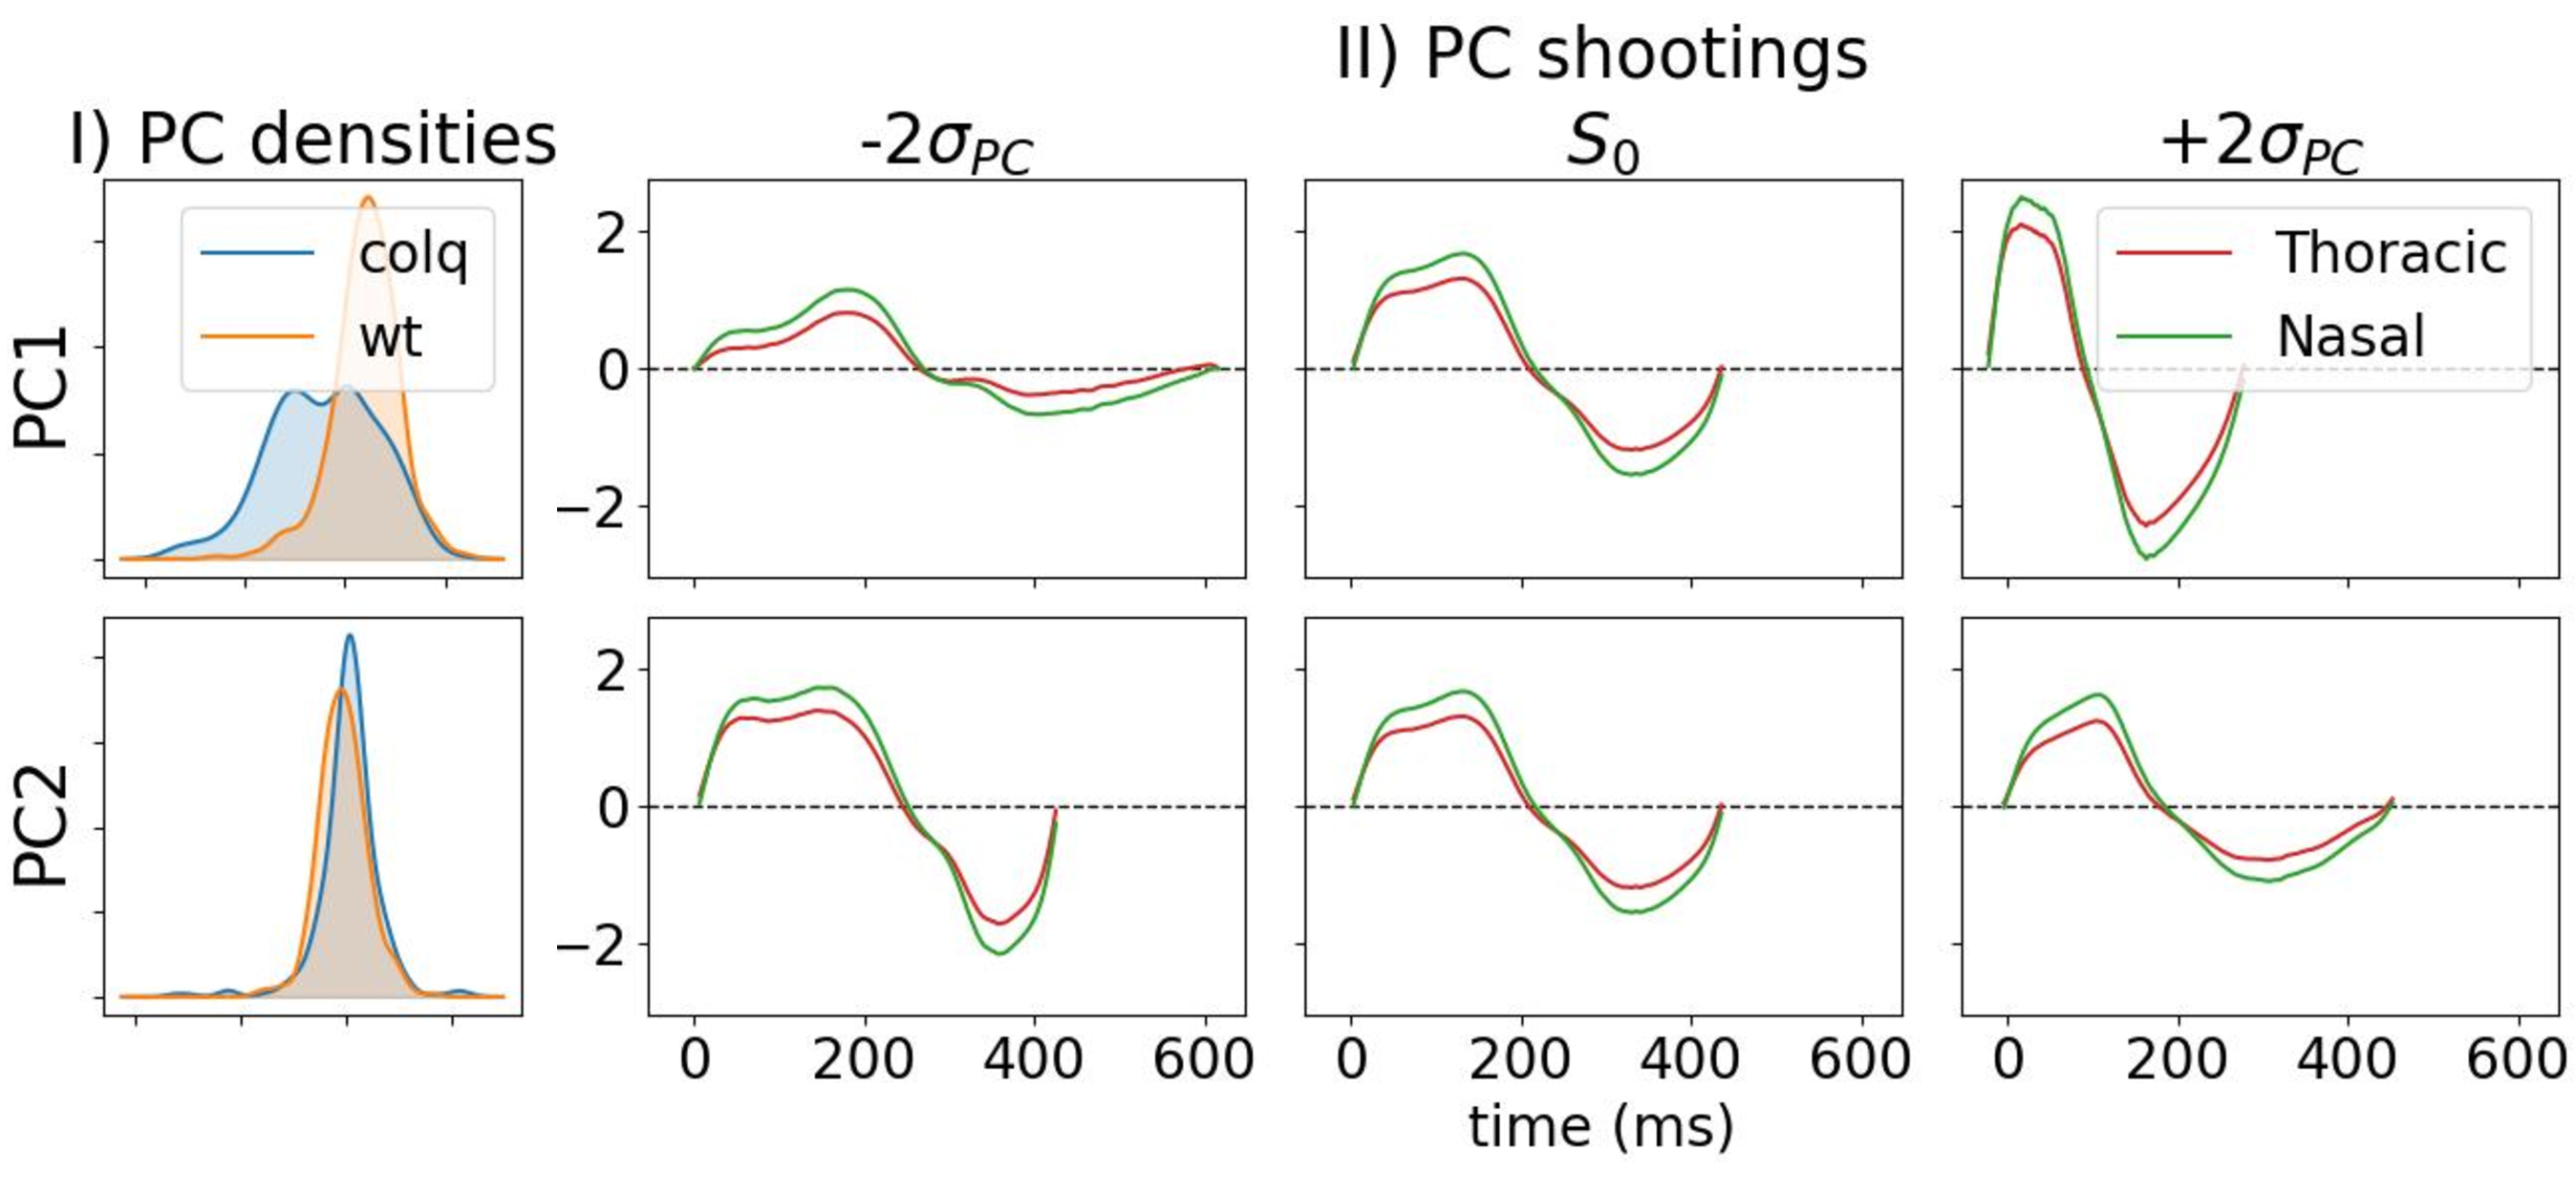
\includegraphics[width = \textwidth]{pictures/ts_ddmm_shooting.pdf}
    \caption{TS-LDDMM}
    \label{fig:ts-lddmm shooting}
  \end{subfigure}
  \begin{subfigure}[b]{0.49\textwidth}
    \centering
    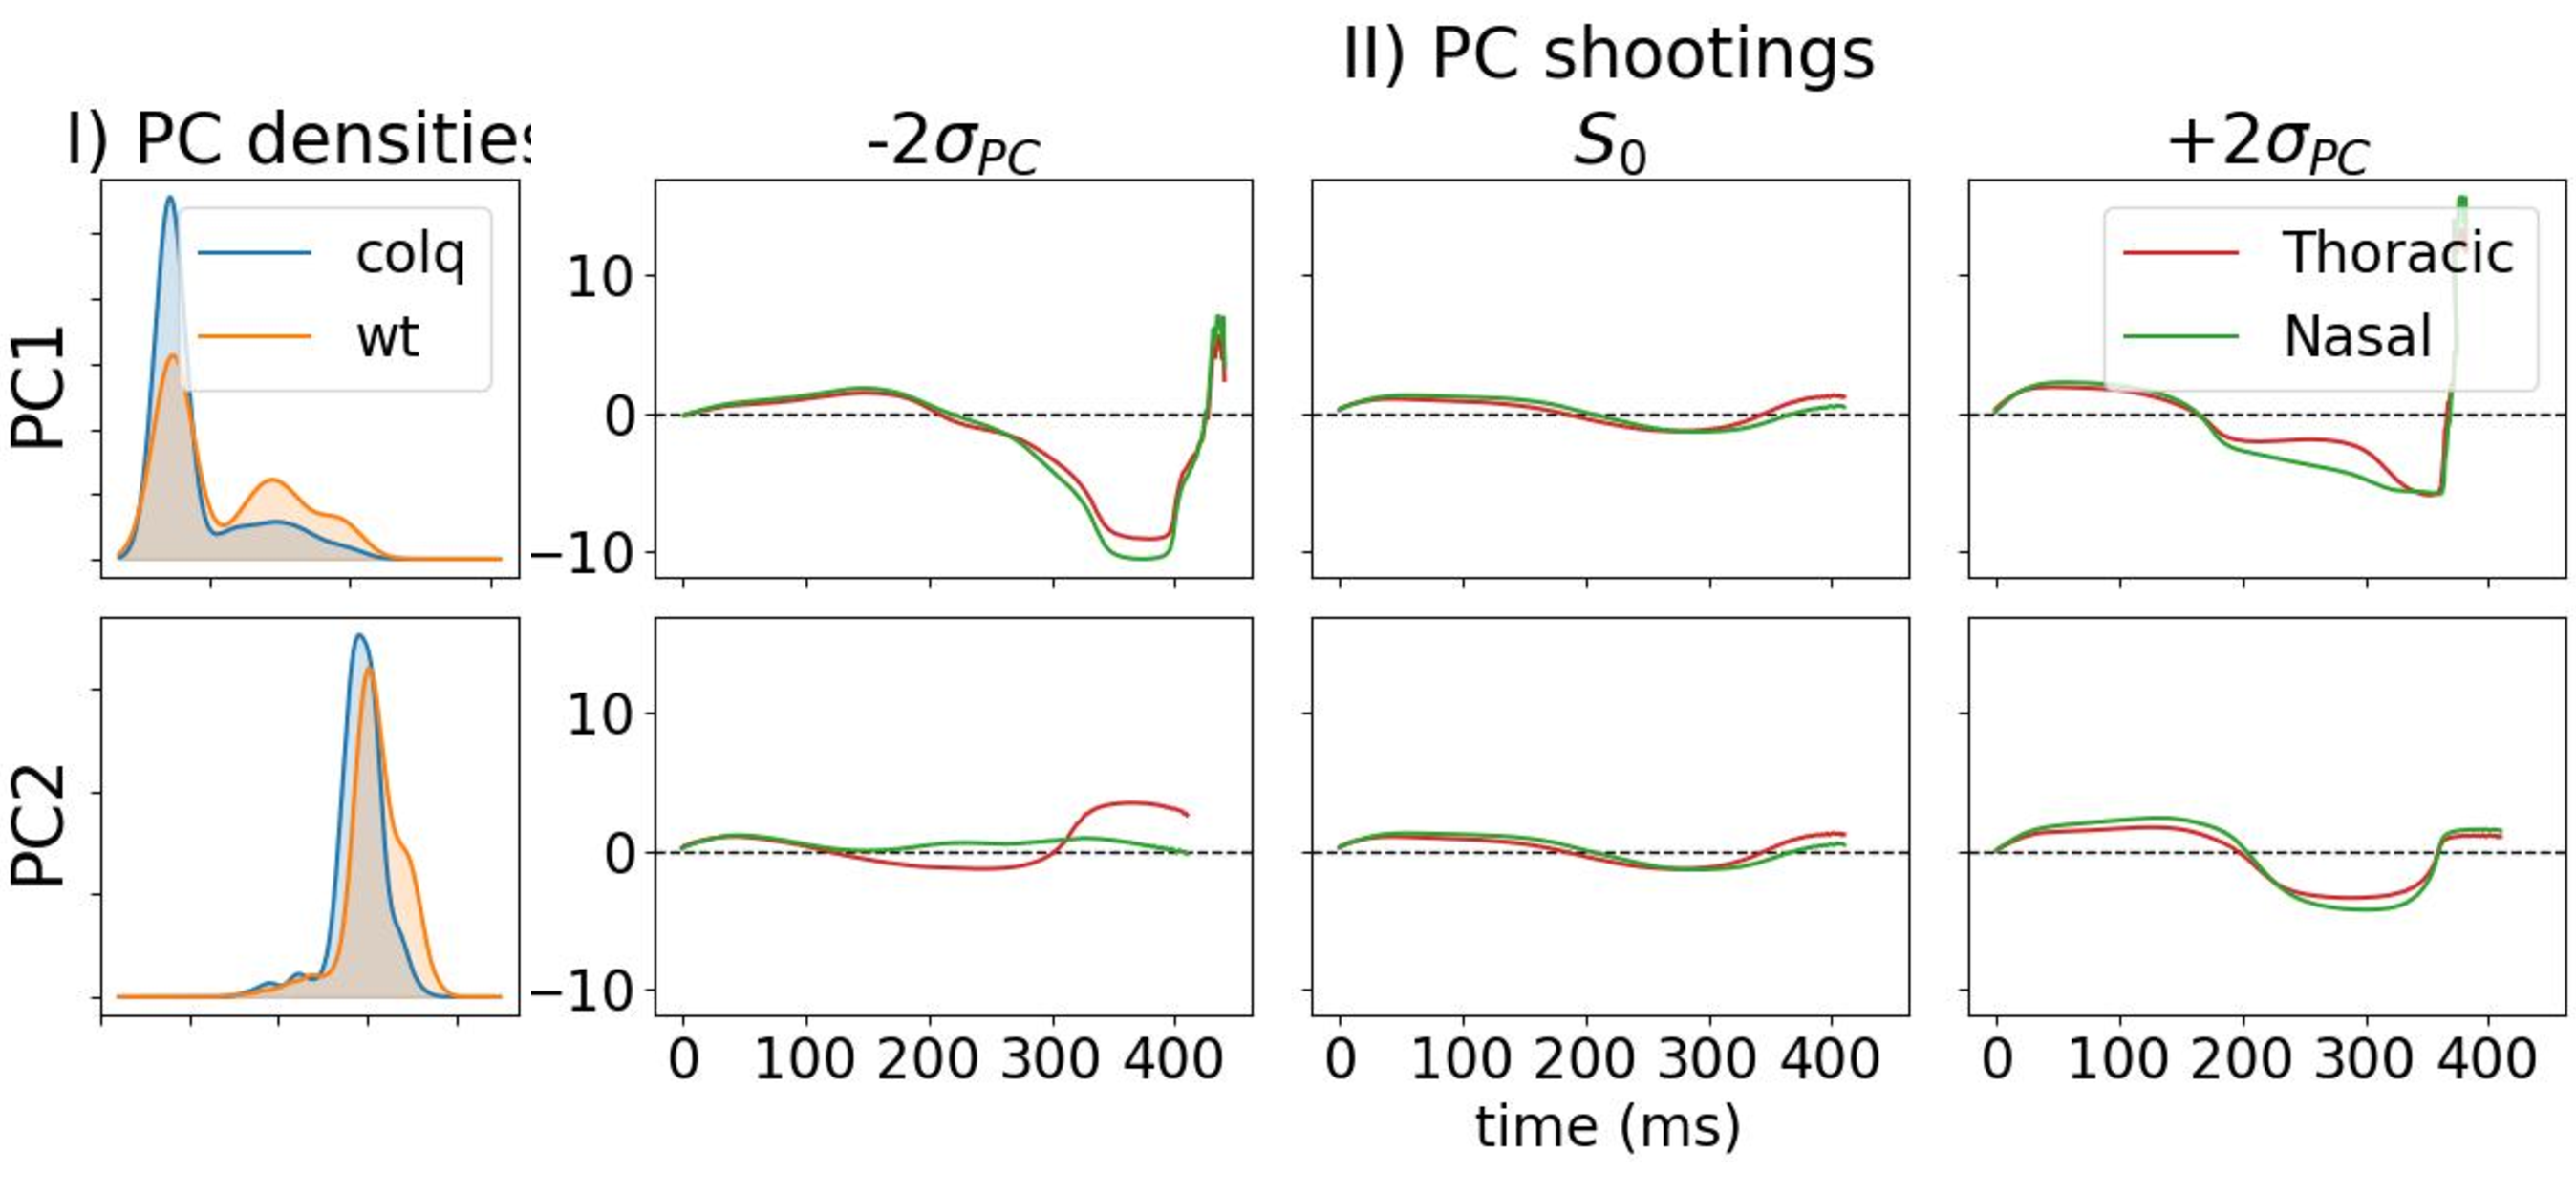
\includegraphics[width = \textwidth]{pictures/lddmm_shooting.pdf}
    \caption{LDDMM}
    \label{fig:lddmm shooting}
  \end{subfigure}
  \caption{Analysis of the two principal components (PC) related to mice' respiratory cycles before exposure for TS-LDDMM \Cref{fig:ts-lddmm shooting}, and LDDMM \Cref{fig:lddmm shooting}.
  In both cases, I) displays PC densities according to mice genotype and II) displays  deformations of the reference graph $S_0$ along each PC.}
  \label{fig:exp1}
\end{figure*}

\begin{wrapfigure}{r}{0.50\textwidth}
  \centering
  \begin{subfigure}[b]{0.16\textwidth}
    \centering
    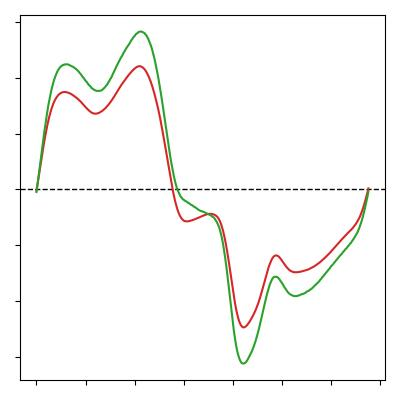
\includegraphics[width = \textwidth]{pictures/exp_1_cycle_example.jpeg}
    \caption{colq cycle}
    \label{fig:colq-cycle}
  \end{subfigure}
  \begin{subfigure}[b]{0.16\textwidth}
    \centering
    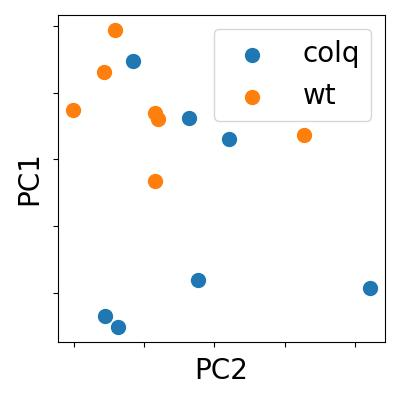
\includegraphics[width = \textwidth]{pictures/exp_1_scatter.jpeg}
    \caption{PC1 vs PC2}
    \label{fig: pcs-scatter}
  \end{subfigure}
  \begin{subfigure}[b]{0.16\textwidth}
    \centering
    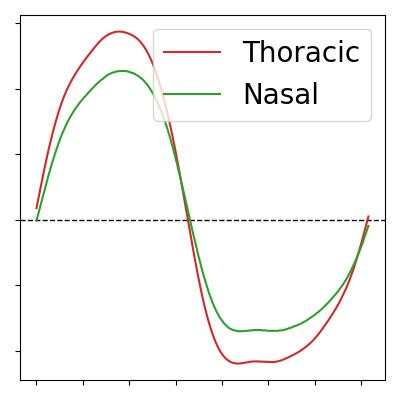
\includegraphics[width = \textwidth]{pictures/exp_1_wt.jpeg}
    \caption{wt cycle}
    \label{fig:wt-reference}
  \end{subfigure}
  \caption{\Cref{fig:colq-cycle} is a \textbf{colq} respiratory cycle. \Cref*{fig: pcs-scatter} displays individual mouse reference respiratory cycle in the TS-LDDMM PC1-PC2 coordinates. \Cref{fig:wt-reference} is a referent respiratory cycle of a \textbf{wt} mouse learned with TS-LDDMM. }
  \vspace{-1em}
\end{wrapfigure}


%the densities of each genotype according to each PC are displayed. In Figure B), the deformations of the reference graph $S_0$ along each PC are given. In Figure D), the graph of reference $S^j$, also called barycenter, related to each mouse, is displayed according to their coordinates on PC1 and PC3. In Figure C) et E), illustrations of respiratory cycles related to mice coming from the \textbf{wt} and \textbf{colq} group are displayed.

%\begin{figure*}[t]
%  \centering
%  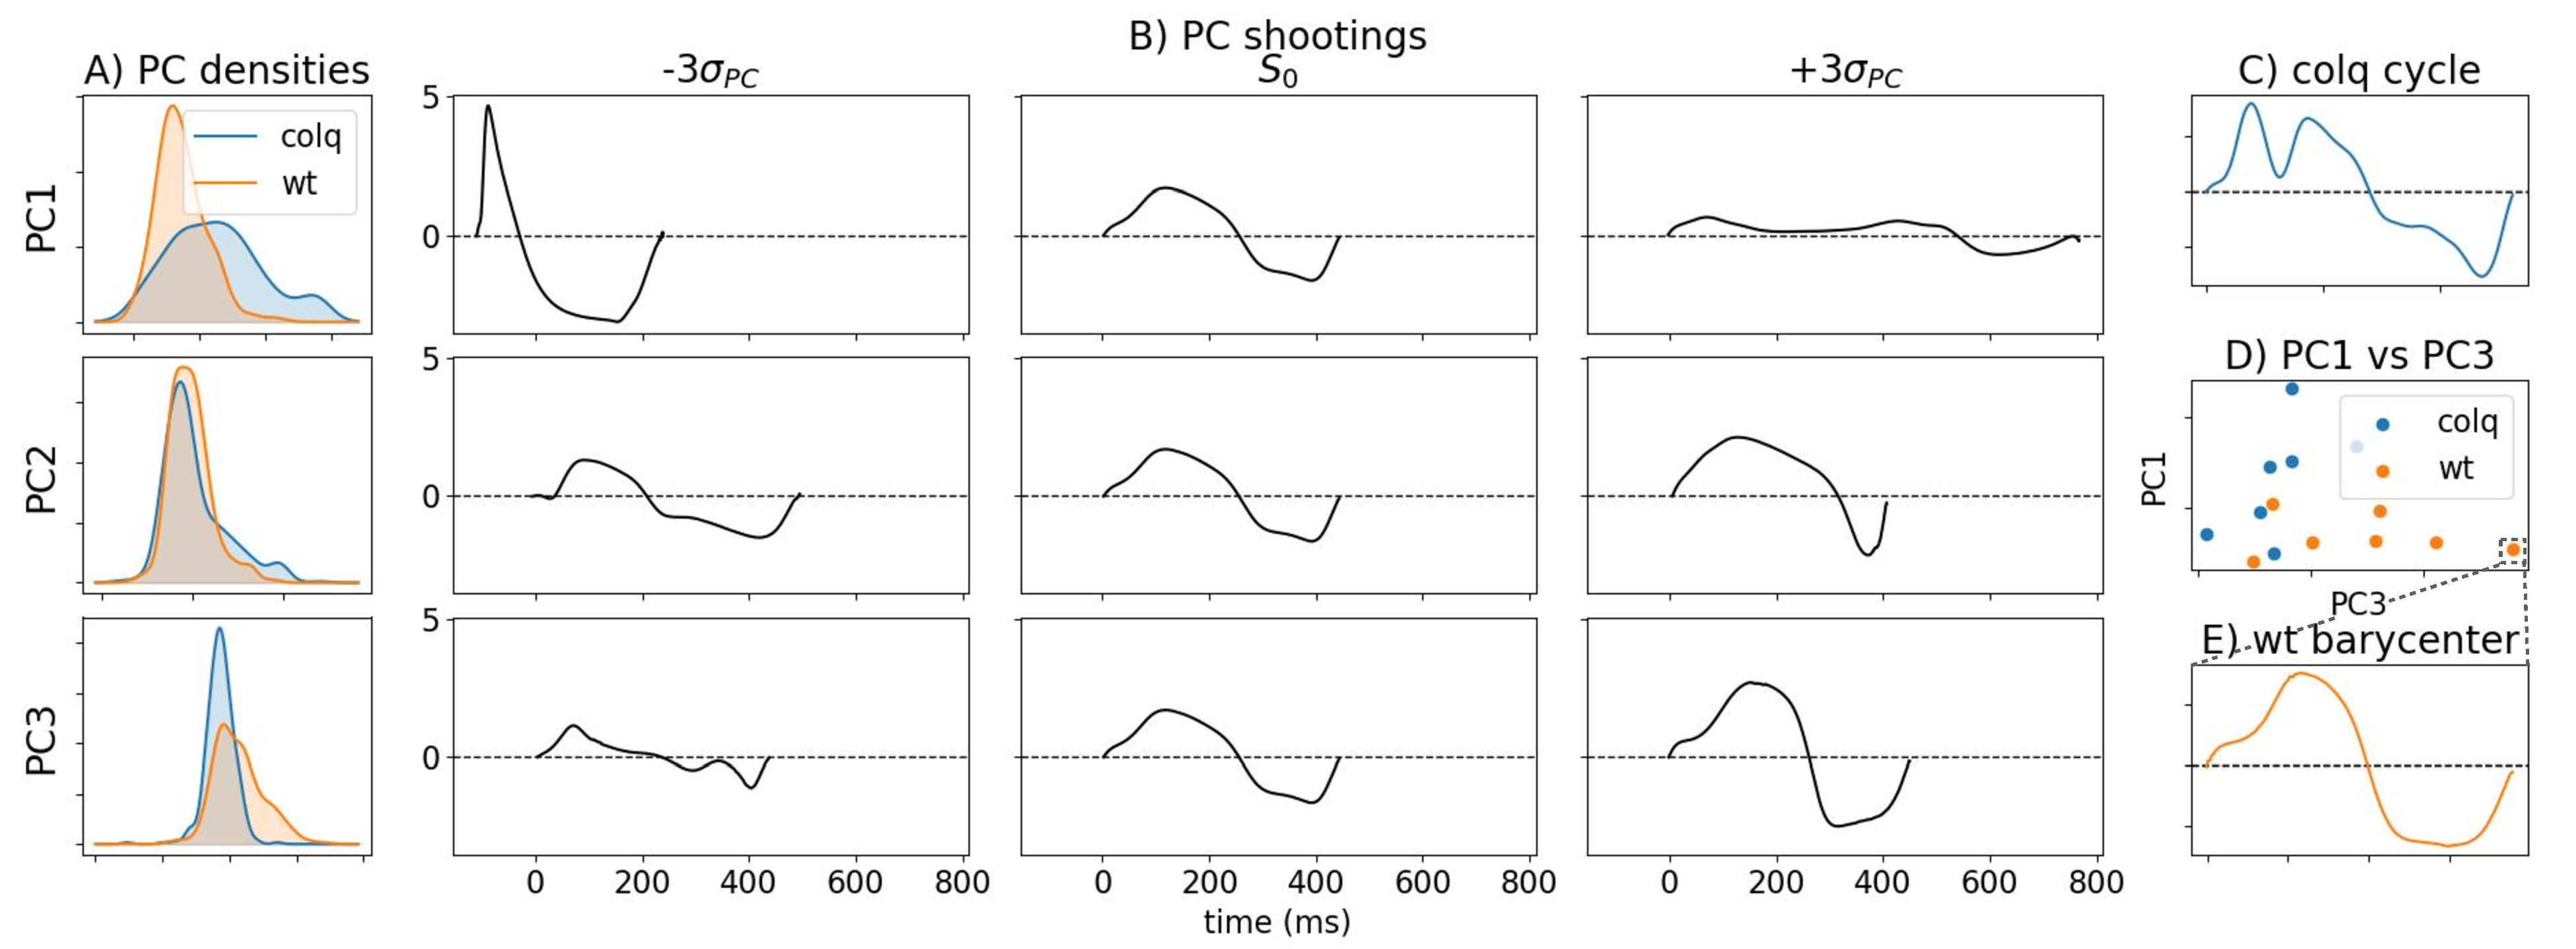
\includegraphics[width=0.95\linewidth]{"./pictures/exp_1_bis.pdf"}
%  \vspace{-1.5em}
%  \caption{Analysis of the two principal components (PC) related to the mice respiratory cycles before exposure for TS-LDDMM \Cref{fig:ts-lddmm shooting}.
%  In Figure A), the densities of each genotype according to each PC are displayed. In Figure B), the deformations of the reference graph $S_0$ along each PC are given. In Figure D), the graph of reference $S^j$, also called barycenter, related to each mouse, is displayed according to their coordinates on PC1 and PC3. In Figure C) et E), illustrations of respiratory cycles related to mice coming from the \textbf{wt} and \textbf{colq} group are displayed.  }
%  \label{fig:exp_1_PCA}
%  %\vspace{-1em}
%\end{figure*}

This experiment highlights the \textit{interpretability} of TS-LDDMM representation for studying the inter-individual variability in time series biomedical datasets. We consider a multivariate time series dataset that accounts for mice's nasal and thoracic airflow evolution when exposed to an irritant molecule altering respiratory functions \cite{nervo2019respiratory}.
The dataset is divided into two groups, one composed of 7 control mice (\textbf{wt}) and the other of 7 mice (\textbf{colq}) deficient in an enzyme involved in the control of respiration. For each mouse, airflows were recorded for 15 to 20 minutes before exposure to the irritant molecule and then for 35 to 40 minutes. A complete 
description of the dataset is given in the \Cref{appendix:mouse_dataset}.

\paragraph{Result summary.} By comparing the shape of individual respiratory cycles, we show that TS-LDDMM features can encode genotype distinctive breathing behaviors and their evolution after exposure to the irritant molecule. 

\paragraph{Protocol.} For both experiments and representations (TS-LDDMM and LDDMM), we derive the reference respiratory cycle's graph $S_0$ and the representations $(\alpha_j)_{j\in[N]}$ related to $N$ respiratory cycles extracted according to the procedure \cite{germain2023unsupervised} by solving  \eqref{eq:general_optimization_problem}. Then, we perform a kernel PCA on the initial velocity field $\left(v_0(\alpha_j,S_0)\right)_{j\in[N]}\in \msv^{N_1}$ defined in \eqref{eq:def_v0} to breathing behavior. The first experiment includes $N_1 = 700$ respiratory cycles collected before exposure. The second experiment includes $N_2 = 1400$ respiratory cycles with 25\% (resp. 75\%) before (resp. after) exposure. \Cref{appendix: mice_exp_setting} describes methods settings. Essentially, varifold losses are identical for both methods, and the velocity field kernels are set to encompass time and space scales. 


\paragraph{Breathing behaviors before exposure.} We focus on the analysis of the two first Principal Components (PC) for TS-LDDMM (\Cref{fig:ts-lddmm shooting}), and LDDMM (\Cref{fig:lddmm shooting}). A respiratory cycle is an inspiration (positive flow) followed by an expiration (negative flow); \Cref{fig:wt-reference} displays an example of \textbf{wt} mouse respiratory cycle. \Cref{fig:exp1} shows that principal components learned with TS-LDMM lead to deformations that remain respiratory cycles, while deformations learned with LDDMM are challenging to interpret as respiratory cycles. The LDDMM velocity field kernel is a Gaussian anisotropic kernel that accounts for time and space scales; however, the entanglement of time and space dimensions in the kernel does not guarantee the graph structure, and it makes the convergence of the method difficult (relative varifold loss error: TS-LDDMM: 0.06, LDDMM: 0.11). Regarding TS-LDDMM, \Cref{fig:ts-lddmm shooting} shows its principal components refer to different types of deformations. By interpreting \Cref{fig:ts-lddmm shooting}: PC1 accounts for time warping, PC2 expresses the trade-off between inspiration and expiration duration. Compared to \textbf{wt} mice, the distribution of \textbf{colq} mice feature along the PC1 axis has a heavy left tail, and the associated deformation (-2 $\sigma_{\text{PC}}$) shows an inspiration with two peaks. \Cref{fig:colq-cycle} shows an example of such respiratory cycles, which may be caused by motor impairment due to enzyme deficiency, \cite{germain2023unsupervised}. Finally, \Cref{fig: pcs-scatter} shows that PC1 and PC2 capture the main differences between the two groups as their respective reference graphs $S^j$ are located in different parts of the space. 

\begin{figure*}[t]
  \centering
  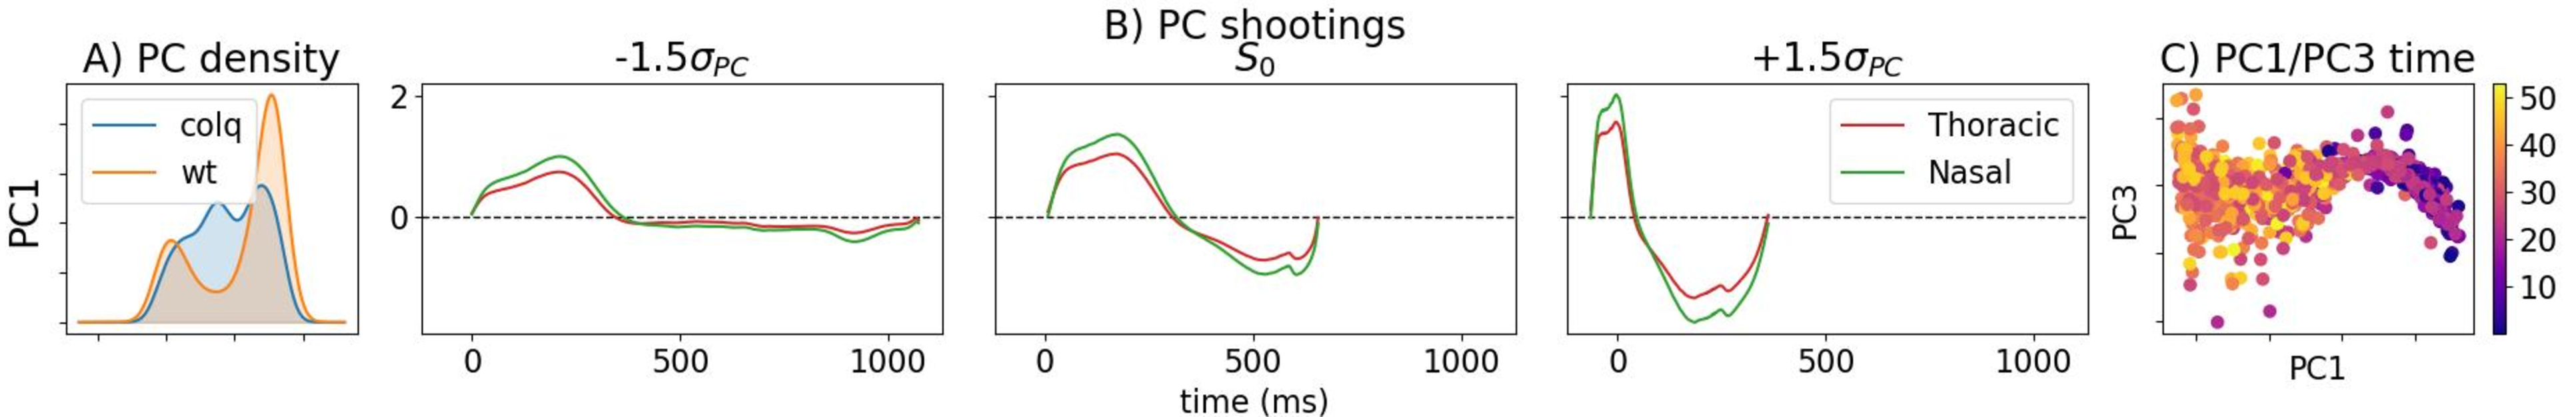
\includegraphics[width=0.95\linewidth]{"./pictures/exp2.pdf"}
  \caption{Analysis of the first Principal Component (PC1) related to mice' respiratory cycles before and after exposure for TS-LDDMM. Figure A) displays PC densities according to mice genotype, Figure B) displays  deformations of the reference graph $S_0$ along PC1, and Figure C) displays respiratory cycles with respect to time in PC1 and PC3 coordinates}
  \label{fig:exp_2_PCA}
  \vspace{-1.5em}
\end{figure*}

\paragraph{Breathing behaviors' evolution after exposure to the irritant molecule} 
TS-LDDMM representation features are learned on a dataset that includes respiratory cycles before and after exposure. \Cref{fig:exp_2_PCA} displays the first principal component PC since it encodes the effect of the irritant molecule as depicted in \Cref{fig:exp_2_PCA}-C) (the exposure occurs at 20 minutes). \Cref{fig:exp_2_PCA}-B) shows that the deformation (-1.5 $\sigma_{\text{PC}}$) leads to longer respiratory cycles that include a pause between inspiration and expiration as observed in \cite{germain2023unsupervised}. Conjointly, \Cref{fig:exp_2_PCA}-A) shows a bimodal distribution for \textbf{wt} mice whereas \textbf{wt}' distributions before exposure were unimodal (\Cref{fig:ts-lddmm shooting}). Indeed, the irritant molecule inhibits the action of the deficient enzyme, \textbf{wt} mice strongly react to the irritant molecule, whereas \textbf{colq} mice better adapt due to their deficiency \cite{germain2023unsupervised}.
%Secondly, we compare breathing behaviors before and after exposure to observe the impact of the irritant molecule.
% We follow the same procedure as for before exposure, but we take $N_2=1400$ respiratory cycles extracted according 
% to the procedure CITE....
% In \Cref{fig:exp_2_PCA}, we focus on the first Principal Component (PC) since it encodes the effect of the irritant molecule as demonstrated on Figure \ref{fig:exp_2_PCA}-C) (exposure at time 20).
% We observe on \Cref{fig:exp_2_PCA}-B) that after exposure the mouse have longuer breath such that the expiration is longuer than inspiration.
%  Moreover, we deduce from Figure \ref{fig:exp_2_PCA}-A) that \textbf{colq} are more constant in their breath compared to \textbf{wt} after exposure.
%
% In Figure REF, we 
% also display the reference respiratory cycle S0 and its deformations in the principal component directions.
%  Additionally, we learn each mouse's reference respiratory cycle and represent them in the first and third PC coordinates system in Figure REF. 
\vspace{-1ex}

\section{Related Works}
\vspace{-1ex}
Shape analysis focuses on statistical analysis of mathematical objects invariant under some deformations like rotations, dilations, or time parameterization.
 The main idea is to represent these objects in a complete Riemannian manifold $(\mathcal{M},\mathbf{g})$ with a metric $\mathbf{g}$ adapted to the geometry of the problem \cite{miller2006geodesic}.
 Then, any set of points in $\mathcal{M}$ can be represented as points in the tangent space of their Frechet mean $\mathbf{m}_0$ \cite{pal2017riemannian,le2001locating} by considering their logarithms.
 The goal is to find a well-suited Riemannian structure according to the nature of the studied object.
 
 LDDMM framework is a relevant shape analysis tool to represent curves as depicted in \cite{glaunes2008large}. However, graphs of time series are a well-structured type of curve due to the inclusion of the temporal dimension that requires specific care (\Cref{fig:diffeo}).
 In a similar vein, Qiu \textit{et al} \cite{qiu2009time} proposes a method for tracking anatomical shape changes in serial images using LDDMM. They include temporal evolution, but not for the same purpose: the aim is to perform longitudinal modeling of brain images.

 Leaving the LDDMM representation, the results of \cite{srivastava2010shape,heo2024logistic} address the representation of curves with the Square-Root Velocity (SRV) representation.
 However, the SRV representation is applied after reparametrization of the temporal dimension of the unit length segment.
 Consequently, the graph structure of the time series is not respected, and the original time evolution of the time series is not encoded in the final representation.
 Very recently, in a functional data analysis framework, a paper \cite{wu2024shape} (Shape-FPCA) improved by representing the original time evolution.
 Nevertheless, this method is made for \textit{continuous objects} and only applies to time series of \textit{same length}, making the estimation more sensitive to noise.

 Balancing between discrete and continuous elements is a challenging task.
 In the deep learning literature \cite{chen2018neural, kidger2020neural, tzen2019neural, jia2019neural, liu2019neural, ansari2023neural}, Neural Ordinary Differential Equations (Neural ODEs) \cite{chen2018neural} learn continuous latent representations using a vector field parameterized by a neural network, serving as a continuous analog to Residual Networks \cite{zagoruyko2016wide}.
 This approach was further enhanced by Neural Controlled Differential Equations (Neural CDEs) \cite{kidger2020neural} for handling irregular time series, functioning as continuous-time analogs of RNNs \cite{schuster1997bidirectional}.
 Extending Neural ODEs, Neural Stochastic Differential Equations (Neural SDEs) introduce regularization effects \cite{liu2019neural}, although optimization remains challenging.
 Leveraging techniques from continuous-discrete filtering theory, Ansari et al. \cite{ansari2023neural} applied successfully Neural SDEs to irregular time series.
 Oh \textit{et al.} \cite{oh2024stable} improved these results by incorporating the concept of controlled paths into the drift term, similar to how Neural CDEs outperform Neural ODEs.
 With TS-LDDMM, the representation is also derived from an ODE, but the velocity field is parameterized with kernels and optimized to have a minimal norm, which enhances interpretability.

 All these state-of-the-art methods previously mentionned \cite{glaunes2008large,oh2024stable,wu2024shape,heo2024logistic} are compared to TS-LDDMM in \Cref{appendix: robustness} and \Cref{appendix: shape_classification}.
 \vspace{-1ex}
  \section{Limitations and conclusion}
  \vspace{-1ex}
  \label{sec:limitations}
  
  This paper proposes a feature representation method, TS-LDDMM, designed for 
shape comparison on homogeneous time series datasets. We show on a real dataset 
its ability to study, with high interpretability, the inter-individual shape 
variability. As an unsupervised approach, it is user-friendly and enables knowledge 
transfer for different supervised tasks such as classification.

Although TS-LDDMM 
is already competitive for classification, its performances can be leveraged on 
more heterogeneous datasets using a hierarchical clustering extension, which is relegated for future work. 
%   While TS-LDDMM performs well on shape-based datasets, it assumes a certain degree of homogeneity with the existence of a reference time series graph$\msg_0$.
%  Extending TS-LDDMM to more heterogeneous datasets using clustering is ongoing work.

 TS-LDDMM employs kernel computations, which require specific libraries (e.g., KeOps \cite{charlier2021kernel}) to be efficient and scalable.
 However, in our experiments, the time complexity of TS-LDDMM is comparable to that of competitors.
 It is clear that TS-LDDMM needs to be extended to handle very large datasets with high-dimensional time series (such as videos).
 
 Additionally, TS-LDDMM requires tuning several hyperparameters, though this is a common requirement among competitors \cite{glaunes2008large, oh2024stable, wu2024shape, heo2024logistic}.
 In future work, adaptive methods are expected to be developed to provide a more user-friendly interface.
  %\color{red} rappeler les limites de la méthodes : petite dimension à cause des kernels, tuner les hyper paramètres correctement, version adaptative}
% \paragraph*{Conclusion}
% \vspace{-1ex}




%\section{Societal impact}
%This paper presents work whose goal is to advance the field of Machine Learning. There are many potential societal consequences of our work, none which we feel must be specifically highlighted here.
% \section{Acknowledgements}

%The TS-LDDMM feature representation proposed in this paper enables us to study the inter-individual variability of shapes in a time series dataset with high interpretability.
%Its unsupervised aspect is user-friendly and enables knowledge transfer for different supervised tasks such as classification.
%Although the method is already competitive,
% its capacity can be leveraged on more heterogeneous datasets using a hierarchical clustering extension.
% This is relegated to future works.

%Applying NF or CNF to our
 %  framework with high dimensional time series is relagated for future works.

% \begin{figure}[ht]
% \vskip 0.2in
% \begin{center}
% \centerline{\includegraphics[width=\columnwidth]{icml_numpapers}}
% \caption{Historical locations and number of accepted papers for International
% Machine Learning Conferences (ICML 1993 -- ICML 2008) and International
% Workshops on Machine Learning (ML 1988 -- ML 1992). At the time this figure was
% produced, the number of accepted papers for ICML 2008 was unknown and instead
% estimated.}
% \label{icml-historical}
% \end{center}
% \vskip -0.2in
% \end{figure}


% \begin{algorithm}[tb]
%    \caption{Bubble Sort}
%    \label{alg:example}
% \begin{algorithmic}
%    \STATE {\bfseries Input:} data $x_i$, size $m$
%    \REPEAT
%    \STATE Initialize $noChange = true$.
%    \FOR{$i=1$ {\bfseries to} $m-1$}
%    \IF{$x_i > x_{i+1}$}
%    \STATE Swap $x_i$ and $x_{i+1}$
%    \STATE $noChange = false$
%    \ENDIF
%    \ENDFOR
%    \UNTIL{$noChange$ is $true$}
% \end{algorithmic}
% \end{algorithm}






